% A reader's guide to "Too Fast to Read": what the paper says, what holds up,
% and what to do with it.   Build:  latexmk -pdf handout.tex
\documentclass[11pt,letterpaper]{article}
\usepackage[T1]{fontenc}
\usepackage[utf8]{inputenc}
\usepackage{mathpazo}
\usepackage{tgpagella}
\usepackage[scale=0.90]{tgheros}
\usepackage[scale=0.92]{tgcursor}
\linespread{1.06}
\usepackage[letterpaper,top=1.1in,bottom=1.15in,left=1.2in,right=1.2in,headheight=15pt,headsep=18pt,footskip=32pt]{geometry}
\usepackage[protrusion=true,expansion=true]{microtype}
\usepackage{amsmath,amssymb,mathtools,bm}
\usepackage[table]{xcolor}
\usepackage{booktabs,tabularx,longtable,array,multirow,makecell}
\usepackage{graphicx}
\usepackage[font=small,labelfont={bf,sf},labelsep=period,skip=6pt]{caption}
\usepackage{enumitem}
\usepackage[most]{tcolorbox}
\usepackage{tikz}
\usetikzlibrary{arrows.meta,positioning,calc,fit,backgrounds,shapes.misc}
\usepackage{fancyhdr}
\usepackage{titlesec}
\usepackage{parskip}
\usepackage{pifont}
\usepackage{needspace}

% ---------------------------------------------------------------- colours
\definecolor{hblue}{HTML}{2A78D6}
\definecolor{hbluedark}{HTML}{104281}
\definecolor{horange}{HTML}{EB6834}
\definecolor{haqua}{HTML}{1BAF7A}
\definecolor{haquadark}{HTML}{0B6B49}
\definecolor{ink}{HTML}{0B0B0B}
\definecolor{inktwo}{HTML}{52514E}
\definecolor{muted}{HTML}{898781}
\definecolor{gridc}{HTML}{E1E0D9}
\definecolor{axisc}{HTML}{C3C2B7}
\definecolor{paperc}{HTML}{F4F3EF}
\definecolor{stgood}{HTML}{0CA30C}
\definecolor{stgooddark}{HTML}{006300}
\definecolor{stwarn}{HTML}{FAB219}
\definecolor{stserious}{HTML}{EC835A}
\definecolor{stcrit}{HTML}{D03B3B}
\definecolor{stcritdark}{HTML}{9E2424}

\usepackage[colorlinks=true,linkcolor=hbluedark,urlcolor=hbluedark,citecolor=hbluedark,
  bookmarksnumbered=true,pdftitle={A reader's guide to Too Fast to Read},pdfauthor={}]{hyperref}

% ---------------------------------------------------------------- layout
\graphicspath{{figures/}}
\setlist{itemsep=2pt,topsep=3pt,parsep=0pt,leftmargin=1.5em}
\renewcommand{\arraystretch}{1.2}
\newcolumntype{L}{>{\raggedright\arraybackslash}X}
\newcolumntype{P}[1]{>{\raggedright\arraybackslash}p{#1}}
\setcounter{tocdepth}{2}
\setcounter{secnumdepth}{2}
\emergencystretch=1.5em

\titleformat{\section}{\sffamily\bfseries\Large\color{hbluedark}}{\thesection}{0.7em}{}
\titleformat{\subsection}{\sffamily\bfseries\large\color{hbluedark}}{\thesubsection}{0.7em}{}
\titleformat{\subsubsection}{\sffamily\bfseries\normalsize\color{ink}}{}{0em}{}
\titleformat{\paragraph}[runin]{\sffamily\bfseries\small\color{ink}}{}{0em}{}[.]
\titlespacing*{\section}{0pt}{20pt plus 4pt minus 2pt}{6pt}
\titlespacing*{\subsection}{0pt}{14pt plus 3pt minus 2pt}{3pt}
\titlespacing*{\subsubsection}{0pt}{10pt plus 2pt minus 1pt}{1pt}
\titlespacing*{\paragraph}{0pt}{6pt plus 2pt}{0.6em}

\pagestyle{fancy}
\fancyhf{}
\renewcommand{\sectionmark}[1]{\markright{\thesection\enspace #1}}
\fancyhead[L]{\sffamily\footnotesize\color{muted}A reader's guide to \emph{Too Fast to Read}}
\fancyhead[R]{\sffamily\footnotesize\color{muted}\nouppercase{\rightmark}}
\fancyfoot[C]{\sffamily\footnotesize\color{muted}\thepage}
\renewcommand{\headrulewidth}{0.3pt}
\renewcommand{\headrule}{{\color{axisc}\hrule width\headwidth height\headrulewidth}}

% Parts: a new page with a title and a short statement of purpose.
\newcounter{hpart}
\newcommand{\handoutpart}[2]{%
  \clearpage\refstepcounter{hpart}%
  \addcontentsline{toc}{part}{Part \Roman{hpart}.\enspace #1}%
  \markright{Part \Roman{hpart}}%
  \vspace*{0.6in}%
  {\sffamily\bfseries\large\color{hblue}PART \Roman{hpart}\par}\vspace{4pt}%
  {\sffamily\bfseries\fontsize{26}{30}\selectfont\color{hbluedark}#1\par}\vspace{10pt}%
  {\color{hblue}\hrule height 1.2pt}\vspace{14pt}%
  {\large\color{inktwo}#2\par}\vspace{0.3in}}

% ---------------------------------------------------------------- boxes
\tcbset{hbase/.style={enhanced,breakable,parbox=false,boxrule=0pt,frame hidden,arc=0pt,outer arc=0pt,
  left=11pt,right=10pt,top=7pt,bottom=7pt,before skip=10pt plus 2pt,after skip=10pt plus 2pt,lines before break=4}}
\newtcolorbox{keybox}[1][Key point]{hbase,colback=hblue!6,borderline west={3pt}{0pt}{hblue},
  before upper={{\sffamily\bfseries\small\color{hbluedark}#1}\par\vspace{1pt}}}
\newtcolorbox{critbox}[1][Problem]{hbase,colback=stcrit!5,borderline west={3pt}{0pt}{stcrit},
  before upper={{\sffamily\bfseries\small\color{stcritdark}#1}\par\vspace{1pt}}}
\newtcolorbox{ideabox}[1][Idea]{hbase,colback=haqua!8,borderline west={3pt}{0pt}{haqua},
  before upper={{\sffamily\bfseries\small\color{haquadark}#1}\par\vspace{1pt}}}
\newtcolorbox{notebox}[1][How we know]{hbase,colback=paperc,borderline west={3pt}{0pt}{axisc},
  fontupper=\small,before upper={{\sffamily\bfseries\footnotesize\color{inktwo}#1}\par\vspace{1pt}}}
% A result of the paper: name, title, status tag; lower part for plain words and the review.
\newtcolorbox{resultbox}[3]{enhanced,breakable,parbox=false,colback=white,colframe=axisc,boxrule=0.5pt,
  arc=1.5pt,left=9pt,right=9pt,top=6pt,bottom=6pt,middle=5pt,lines before break=3,
  before skip=10pt plus 2pt,after skip=10pt plus 2pt,
  colbacktitle=paperc,coltitle=ink,fonttitle=\sffamily\small,toptitle=3pt,bottomtitle=3pt,titlerule=0.4pt,
  title={\textbf{#1}\enspace\textcolor{inktwo}{#2}\hfill #3},
  fontlower=\small,segmentation style={solid,draw=gridc,line width=0.5pt}}
\newcommand{\inwords}{{\sffamily\bfseries\footnotesize\color{hbluedark}IN PLAIN WORDS}\enspace}
\newcommand{\why}{{\sffamily\bfseries\footnotesize\color{inktwo}WHY}\enspace}
\newcommand{\role}{{\sffamily\bfseries\footnotesize\color{inktwo}ROLE}\enspace}
\newcommand{\review}{{\sffamily\bfseries\footnotesize\color{stcritdark}AFTER REVIEW}\enspace}

% Status tags (always a label, never colour alone).
\newcommand{\sttag}[3]{\tcbox[on line,boxsep=0pt,left=4pt,right=4pt,top=2pt,bottom=2pt,arc=2pt,
  boxrule=0pt,colback=#1,colframe=#1]{\sffamily\bfseries\fontsize{7}{8}\selectfont\color{#2}\MakeUppercase{#3}}}
\newcommand{\tsolid}{\sttag{stgood}{white}{solid}}
\newcommand{\trepair}{\sttag{stwarn}{ink}{needs repair}}
\newcommand{\tfragile}{\sttag{stserious}{white}{fragile}}
\newcommand{\tassumed}{\sttag{stserious}{white}{assumed}}
\newcommand{\tfails}{\sttag{stcrit}{white}{does not hold up}}
\newcommand{\tinert}{\sttag{stcrit}{white}{never operates}}
\newcommand{\tuntested}{\sttag{muted}{white}{untested}}
\newcommand{\tminor}{\sttag{muted}{white}{side result}}

% ---------------------------------------------------------------- maths
\newcommand{\E}{\mathbb{E}}
\newcommand{\R}{\mathbb{R}}
\newcommand{\Phat}{\hat P}
\newcommand{\vhat}{\hat v}
\newcommand{\eps}{\varepsilon}
\newcommand{\dd}{\mathrm{d}}
\newcommand{\EE}{\mathcal{E}}
\newcommand{\Pm}{P^{m}}
\newcommand{\thF}{\theta_F}
\newcommand{\etaF}{\eta_F}
\newcommand{\yes}{\textcolor{stgooddark}{\ding{51}}}
\newcommand{\no}{\textcolor{stcritdark}{\ding{55}}}

\begin{document}
% ------------------------------------------------------------------ title page
\thispagestyle{empty}
\vspace*{0.9in}
{\sffamily\bfseries\large\color{hblue}A READER'S GUIDE TO\par}
\vspace{6pt}
{\sffamily\bfseries\fontsize{34}{38}\selectfont\color{hbluedark}Too Fast to Read\par}
\vspace{8pt}
{\sffamily\Large\color{inktwo}Topic Choice and the Incidence of Research Tools\par}
\vspace{18pt}
{\color{hblue}\hrule height 1.4pt}
\vspace{18pt}
{\Large What the paper says, what holds up, and what to do with it\par}
\vspace{0.5in}

\begin{tabularx}{\textwidth}{@{}P{1.25in}L@{}}
\textsf{\small\color{muted}SUBJECT} & The draft of October 2026: 66 pages, three theorems, five lemmas, fourteen propositions, five facts, six empirical designs. \\[3pt]
\textsf{\small\color{muted}PURPOSE} & To explain the whole paper to someone who has not read it, to record every finding of a systematic review of it, and to set out the ideas for making it one coherent paper. \\[3pt]
\textsf{\small\color{muted}BASIS} & An AI-assisted review: five independent readings of the draft, re-checks that recomputed the technical findings from the paper's own code and data, and four alternative designs of the paper scored by three reviewers. \\[3pt]
\textsf{\small\color{muted}DATE} & 11 November 2026 \\
\end{tabularx}

\vfill
\begin{keybox}[The handout in five sentences]
The draft has one good idea: \emph{entry is the margin on which science adjusts, and the price of entering a topic is reading its literature.}
It presents this idea as four separate results, and the two it puts in the headline are the two that its evidence does not test.
The parts of the theory are sound, but the central step, the headline numbers and the title result do not survive a check against the paper's own code.
One coherent paper is in the material: \emph{more researchers open new topics, while faster researchers first thicken the topics they are already in.}
The first half is the paper's best fact; the second half can be tested now, because output per author on arXiv jumped by 11--14\% in 2026 after seven flat years.
\end{keybox}
\vspace{0.3in}
\clearpage

% ------------------------------------------------------------------ one page
\section*{The handout in one page}
\addcontentsline{toc}{section}{The handout in one page}
\markright{The handout in one page}

\textbf{What the paper does.} Researchers choose a topic, split their time between producing and reading, and must read a topic's literature before they can join it. From this the paper derives a payoff that is single-peaked in how crowded a topic is, an equilibrium in which topics behave like cities, a ``speed limit'' beyond which a literature is closed to newcomers, and a theorem on who keeps the gain from a research tool. It adds five facts and six designs from 2.2 million arXiv submissions, and a calibrated model. \emph{Part~I explains all of this from scratch.}

\textbf{What holds up.} The payoff curve (Theorem~1). The rule that inside a topic a tool is worth the time it saves (Lemma~5). The results on incumbents' rents: insiders earn a premium equal to the newcomer's reading cost, and returns rise with crowding even where a topic is too crowded for newcomers (Proposition~5, Corollary~1). The qualitative fact that growth on arXiv opened new topics instead of thickening old ones (Fact~1). Three small magnitudes. The data, the code and the candour of the draft.

\textbf{What does not.} \emph{Part~II gives every finding.} The six most important:
\begin{enumerate}[leftmargin=1.7em]
\item \textbf{The evidence tests the previous version of the paper.} None of the six designs identifies any quantity on which the current headline rests.
\item \textbf{The central theorem needs a repair.} ``Output per researcher equals the value of the frontier'' contradicts the paper's own count of who is producing. With that count, 53--88\% of the gain from a reading tool survives entry, not 14--74\%.
\item \textbf{The headline number is not identified.} ``A production tool is worth 1.3 to 7.2 times a reading tool'' is a range over an assumed parameter.
\item \textbf{The ranking of tools is assumed.} It follows from what explorers are assumed to do, and it reverses under an extension in the paper's own appendix.
\item \textbf{The title result never operates.} No researcher-year in the calibrated economy is above 53\% of the speed limit, and a model without a limit fits equally well.
\item \textbf{Two empirical statements are wrong.} The ``$+7\%$ output for adopters of language models'' is entirely a pre-existing trend. The ``production shock of at most a few percent'' is contradicted by the paper's own data.
\end{enumerate}

\textbf{The ideas.} \emph{Part~III develops them.} The draft's results are four consequences of one mechanism. Because entry is what adjusts, (1) more researchers open new topics, (2) insiders earn a rent, (3) the gain from a tool stays with whoever is not on the entry margin, and (4) faster researchers are absorbed differently from more researchers. The fourth is the new idea. Until 2025 arXiv grew through more authors; in 2026 output per author jumped. The model says the two kinds of growth land in different places, and that can be checked.

\textbf{What to do.} Do not rewrite yet. Run two measurements first: repair and reproduce the main fact, then test where the extra papers of 2026 landed. Let the result choose between a paper on \emph{scale versus speed} and a fallback on the entry margin and the incidence of tools. Shelve the speed limit and the topic life cycles. Retire the title.

\clearpage
\subsection*{How to read the boxes}
\begin{tabularx}{\textwidth}{@{}P{1.55in}L@{}}
\textsf{\small Grey frame} & A result of the paper, stated formally, then in plain words, then what the review found. The tag on the right gives the verdict. \\
\textsf{\small\color{hbluedark}Blue bar} & A point to keep. \\
\textsf{\small\color{stcritdark}Red bar} & A problem found by the review. \\
\textsf{\small\color{haquadark}Green bar} & An idea. \\
\textsf{\small\color{inktwo}Grey bar} & How we know: what was recomputed, and from which file. \\
\end{tabularx}

\medskip
\noindent\begin{tabularx}{\textwidth}{@{}P{1.55in}L@{}}
\tsolid & Rederived or recomputed, and independent of the parts that fail. \\
\trepair & Right idea, wrong statement or wrong number; the repair is known. \\
\tfragile\ \tassumed & Depends on a parameter that nothing measures, or on an assumption that decides the result. \\
\tfails\ \tinert & Contradicted by the paper's own code or data, or without any effect in the calibrated economy. \\
\tuntested\ \tminor & Correct as far as checked, but no evidence bears on it, or nothing else depends on it. \\
\end{tabularx}

\bigskip
{\setlength{\parskip}{0pt}\small\tableofcontents}
\clearpage

\handoutpart{What the paper says}{This part explains the whole draft to a reader who has not opened it: the question, the model built up one piece at a time, every result in formal terms and in plain words, the evidence piece by piece, and the numbers. Each result carries a tag that says what the review in Part~II found, so the two parts can be read side by side.}

\section{The paper in brief}

\subsection{The question}

Science is producing papers faster. Submissions to arXiv more than doubled between 2018 and 2025, and tools based on large language models now speed up both the writing of research and the reading of it. The draft asks what this does to science when researchers are free to choose what they work on. It poses the question in three ways, and Part~II argues that this is its first problem:

\begin{itemize}
\item \emph{Is innovation too fast?} Can a literature grow faster than the people outside it can absorb? (Title and conclusion.)
\item \emph{Will faster production flood science with duplicates, and are better reading tools the remedy?} (First paragraph of the introduction.)
\item \emph{Which research tools raise the output of science in the long run, and through whom?} (Subtitle and the main theorem.)
\end{itemize}

\subsection{The answer the draft gives}

The abstract makes six claims. In plain words:

\begin{enumerate}
\item \textbf{A payoff curve.} What a researcher earns in a topic first rises and then falls with the number of papers the topic produces. More papers mean more to learn from, and also more earlier work that may already contain her project.
\item \textbf{Topics are like cities.} Free choice of topics fills each topic past its best size, as free migration does with cities. New topics play the role of new cities.
\item \textbf{A speed limit.} A newcomer must read a topic's literature before she can contribute. If the literature grows faster than she reads, she never catches up. Such topics are closed, the people inside earn large rents, fast-growing topics overshoot and slow ones never take off.
\item \textbf{Frontier incidence.} In the long run output per researcher equals the value of opening a new topic. So a tool is worth what it adds to that value. Production tools keep almost all of their value; reading tools keep the part that reaches the founders of topics; tools that help newcomers catch up keep least.
\item \textbf{Units matter.} If papers are valued by how much they are read and not by the credit they earn, the ranking of tools reverses.
\item \textbf{Evidence.} On arXiv more volume opens new ground instead of thickening old topics, and ``four arXiv rule changes and design features identify the margins the model relies on.''
\end{enumerate}

The headline number is that, per hour saved, a production tool is worth 1.3 to 7.2 times a reading tool, and that the static gain from a better allocation of researchers to topics is small (about 1\%).

\subsection{How the draft is organised}

\begin{center}\small
\begin{tabularx}{\textwidth}{@{}P{0.9in}P{1.55in}L@{}}
\toprule
Section & Title & What it contains \\
\midrule
1 & Introduction & Three results, four novelty claims, the evidence, related work. \\
2 & Model & Researchers, topics, reading, credit, catch-up, the frontier, equilibrium. Lemmas 1--4. \\
3 & The payoff curve & Theorem 1, Lemma 5 (time shares), Proposition 1. \\
4 & Free topic choice without frictions & Propositions 2--4: equilibrium, the volume elasticity, the planner. \\
5 & Catch-up, the speed limit and rents & Proposition 5, Theorem 2, Corollary 1, Proposition 6. \\
6 & The incidence of research tools & Theorem 3, Corollary 2, Propositions 7--8. \\
7 & Evidence I: the arXiv record & Facts 1--5. \\
8 & Evidence II: arXiv's rules as experiments & Six designs. \\
9 & Quantification & Calibration, fit, magnitudes. \\
10 & Implications & Propositions 9--11: life cycles, stepping on toes, policy. \\
11--12 & Predictions; conclusion & Fifteen predictions. \\
A--D & Appendices & Proofs; eight extensions (Propositions 12--14); numerics; data. \\
\bottomrule
\end{tabularx}
\end{center}

In total: 3 theorems, 5 lemmas, 14 propositions, 2 corollaries, 6 remarks, 5 facts, 6 designs, 15 predictions, 9 tables and 9 figures. The notation table lists 47 symbols and about 30 more are used without being listed.

\subsection{How the draft got here}

The headline has changed with every version, and the evidence has not kept up. This history explains most of what Part~II finds.

\begin{center}\small
\begin{tabularx}{\textwidth}{@{}P{1.2in}LL@{}}
\toprule
Version & Headline & Evidence \\
\midrule
1.\ \emph{When Innovation Is Too Fast: Reading, Writing, and the Crowding of Science} (21~Oct.) & Faster production crowds topics and raises duplication. The payoff curve and the planner's problem. & Descriptive facts from arXiv. \\
2.\ \emph{Faster Writing Scales Science, Better Reading Crowds It} (23~Oct.) & Writing versus reading. Duplication is pinned by entry, not by volume. Gains from reading tools are competed away; gains from production tools are not. & Facts 1--5 and the six designs were written for this version. \\
3.\ \emph{Too Fast to Read: Topic Choice and the Incidence of Research Tools} (28~Oct., current) & A speed limit, and frontier incidence: a tool is worth what it adds to the value of opening a topic. & Unchanged. One word of the evidence sections differs from version~2. \\
\bottomrule
\end{tabularx}
\end{center}

Version~3 was a response to a detailed referee-style critique of the theory in version~2. That critique was right on each point: in version~2 the people who open topics never read and never stayed in them, so reading tools were ``competed away'' by construction; the comparison of writing with reading (26 log points against 0.2) mostly reflected the share of time each activity takes; and the catch-up cost was a linear approximation. Version~3 fixed each of these. In doing so it added a third headline on top of two earlier ones, and it left the empirical half of the paper where it was.

\begin{keybox}[What to keep in mind while reading Part~I]
The draft is best read as four blocks that were written at different times:
(A)~\emph{topics as cities}, with the fact that growth opens new topics;
(B)~\emph{the incidence of tools};
(C)~\emph{catch-up, the speed limit and topic life cycles};
(D)~\emph{arXiv's rule changes as experiments}.
Block~A is the only one in which a theorem meets a measured number. Blocks~B and~C carry the title and the abstract.
\end{keybox}

\section{The model, one piece at a time}\label{sec:model}

\subsection{The world in one picture}

There is a continuum of \emph{topics} and a mass $N$ of \emph{researchers}. Time is continuous and the economy is in a steady state. At any moment a researcher is in one of three situations (Figure~\ref{fig:world}): exploring at the frontier, reading her way into an existing topic, or producing inside a topic. Whenever she is free she picks the better of two options, exploring or joining, and in equilibrium the two are worth the same.

\begin{figure}[h]
\centering
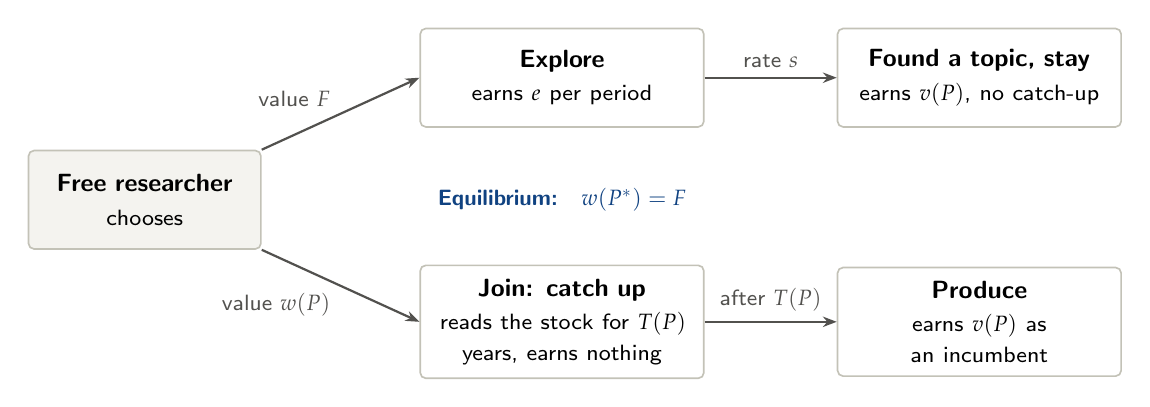
\begin{tikzpicture}[font=\sffamily\small,
  box/.style={draw=axisc,line width=0.6pt,rounded corners=2pt,fill=white,align=center,inner sep=5pt,minimum height=1.25cm,text width=3.25cm},
  arr/.style={-{Stealth[length=5pt]},line width=0.8pt,color=inktwo},
  lab/.style={font=\sffamily\footnotesize,color=inktwo,align=center}]
\node[box,fill=paperc,text width=2.6cm] (free) at (0,0) {\textbf{Free researcher}\\[1pt]{\footnotesize chooses}};
\node[box] (explore) at (5.3,1.55) {\textbf{Explore}\\[1pt]{\footnotesize earns $e$ per period}};
\node[box] (found) at (10.6,1.55) {\textbf{Found a topic, stay}\\[1pt]{\footnotesize earns $v(P)$, no catch-up}};
\node[box] (catch) at (5.3,-1.55) {\textbf{Join: catch up}\\[1pt]{\footnotesize reads the stock for $T(P)$ years, earns nothing}};
\node[box] (prod) at (10.6,-1.55) {\textbf{Produce}\\[1pt]{\footnotesize earns $v(P)$ as an incumbent}};
\draw[arr] (free.north east) -- node[lab,above left=-1pt and 0pt] {value $F$} (explore.west);
\draw[arr] (free.south east) -- node[lab,below left=-1pt and 0pt] {value $w(P)$} (catch.west);
\draw[arr] (explore) -- node[lab,above] {rate $s$} (found);
\draw[arr] (catch) -- node[lab,above] {after $T(P)$} (prod);
\node[lab,color=hbluedark] at (5.3,0) {\textbf{Equilibrium:}\quad $w(P^*)=F$};
\end{tikzpicture}
\caption{A researcher's options. Every spell ends at rate $\rho$ (her career in that topic ends) or $\xi$ (the topic becomes obsolete), and she is then free again. Payoffs are per unit of production speed $a$.}
\label{fig:world}
\end{figure}

Six objects carry the whole model.

\begin{center}\small
\begin{tabularx}{\textwidth}{@{}P{0.55in}P{1.6in}L@{}}
\toprule
Symbol & Name & Meaning \\
\midrule
$a$, $b$ & production and reading speed & Projects produced, and papers read, per year of full-time work. \\
$P$ & density & The flow of papers a topic produces per year. The measure of crowding. \\
$v(P)$ & payoff curve & What an incumbent earns per period in a topic of density $P$, per unit of $a$. \\
$w(P)$ & newcomer's payoff & What a newcomer earns on average over her spell: $v(P)$ scaled down by the time she spends catching up. \\
$F$ & frontier value & What exploring is worth per period. \\
$\EE$ & volume elasticity & By how much density rises when the number of researchers rises by 1\%. \\
\bottomrule
\end{tabularx}
\end{center}

\subsection{Inside a topic: the two jobs of reading}

\subsubsection{Time, production and density}
A researcher has one unit of time per period. She spends a share $x$ producing and a share $r=1-x$ reading. Full-time production yields $a$ projects per period; full-time reading covers $b$ papers. A topic with $n$ producing members therefore receives a flow of
\[
P = a\,x\,n \quad\text{papers per period.}
\]
This flow is the topic's \emph{density}. The paper is explicit that $a$ is research output per unit of production time (doing the research and writing it up), not drafting speed: a tool that drafts text faster raises $a$ only by the share of production time that drafting takes.

Density is a flow. What a researcher learns from, and what can pre-empt her project, is the topic's current literature. What a newcomer must master is the \emph{stock}, the accumulated literature. The distinction is the one between keeping up with a field and getting into it, and it matters only for topics that grow or shrink.

\subsubsection{Job one: reading teaches}
Reading a share $r$ of the time covers $R=br$ papers of the topic's flow. What she reads raises the quality of her own work by a factor $Q(R,P)\ge 1$. The paper assumes (Assumption~1) that nothing is learned without reading or without a literature, that what one can learn is bounded by what one reads, and that $\ln Q$ is jointly concave and supermodular: no increasing returns to reading, and reading is worth more where there is more to read. The running example is
\[
Q(R,P)=\bigl(1+\beta\,h(R,P)\bigr)^{\gamma},\qquad h(R,P)=\frac{RP}{R+P},
\]
where $h$ is close to $R$ when she samples a small part of a rich literature and close to $P$ when she reads a thin one exhaustively.

\subsubsection{Job two: reading protects}
Each earlier paper in the topic \emph{covers} her project with a small probability, so the number of earlier covering papers is Poisson with mean $\theta P$. She catches a covering paper only if she finds it. With reading coverage $c=R/P$ this happens with probability $\varphi(c)$, increasing and concave (Assumption~2); the example is $\varphi(c)=1-e^{-\sigma c}$, where $\sigma$ is search precision. Some overlap cannot be prevented: projects in progress elsewhere arrive at rate $\theta_cP$ and cannot be found in the literature.

Overlap erodes credit. An undetected earlier covering paper removes a share $\lambda$ of the project's credit; a concurrent one removes $\lambda_c$. If she catches a covering paper she either \emph{pivots} to a fresh variant (keeping $1-\kappa_p$) or \emph{proceeds} as a follow-on that cites the earlier paper (keeping a random share $\delta$). She loses $\ell<\lambda$ on average after a detection, so detection is worth $\Delta=\lambda-\ell$.

\begin{resultbox}{Lemma 1}{Credit and overlap}{\tminor}
Expected credit per project is
\[
C(R,P)=\exp\Bigl\{-\theta P\bigl[\lambda-\Delta\,\varphi(R/P)\bigr]-\theta_c\lambda_cP\Bigr\}.
\]
Earlier covering papers that the researcher does not pivot away from (``flagged overlap'') arrive at rate $\theta P[1-(1-q)\varphi]$, where $q$ is the share of detections that proceed. A share $A=q\varphi/[1-(1-q)\varphi]$ of them is \emph{aware}: the later paper cites the earlier one.
\tcblower
\inwords Credit falls exponentially with the number of papers in the topic, and reading slows the fall. The formula also says what the data should show: how often a paper sits very close to an earlier one, and how often it cites it.

\role It connects the model to two observables (the overlap rate and the aware share) and supplies the falling arm of the payoff curve. The paper says that its incidence results do not depend on it.

\review Correct. But the block is quantitatively inert (overlap destroys 2.9\% of credit at the calibrated density), it absorbs most of the paper's empirical effort, and its inputs are soft (\S\ref{sec:crit-evidence}).
\end{resultbox}

\subsubsection{The researcher's problem and the payoff curve}
A researcher in a topic of density $P$ earns $a\,x\,Q\,C$ per period. Dividing by $a$:
\[
g(r,P)=(1-r)\,Q(br,P)\,C(br,P),\qquad v(P)=\max_{r\in[0,1)} g(r,P).
\]
The function $v$ is the \emph{payoff curve}. Production speed scales every payoff and drops out of it. The researcher takes $P$ as given: she ignores that her papers teach her colleagues and that they add to what her colleagues must read.

\begin{resultbox}{Theorem 1}{The payoff curve}{\tsolid}
For any learning and detection technology satisfying the assumptions above:
(i)~$v(0)=1$ and $v(P)\to0$ as $P\to\infty$;
(ii)~$\ln v$ is concave;
(iii)~$v$ rises up to a unique peak $\Phat$ and falls afterwards, with $v(\Phat)>1$;
(iv)~its slope is
\[
\frac{v'(P)}{v(P)}=\underbrace{\partial_P\ln Q}_{\text{more to learn from}}-\underbrace{\theta\bigl[\lambda-\Delta\bigl(\varphi(c^*)-c^*\varphi'(c^*)\bigr)\bigr]-\theta_c\lambda_c}_{\text{more to miss}};
\]
(v)~the optimal reading share $r^*(P)$ rises with density, so papers per researcher fall with density.
\tcblower
\inwords A thin topic gets better as it fills, because there is more to learn from. A crowded topic gets worse as it fills, because more of what you do has already been done and you cannot read it all. In between there is one best size.

\why $\ln g$ is jointly concave in reading time and density. The erosion term is linear in $P$ plus the perspective of the concave function $\varphi$, and perspectives preserve concavity. Maximising a jointly concave function over one argument leaves a concave function of the other. The fall comes from \emph{bounded absorption}: what one person can read and learn is bounded, while the number of papers that may cover her project grows in proportion to the literature.

\review The proof was rederived and holds. Two caveats on its use. The calibrated curve is nearly flat: $v$ lies between 1.78 and 1.98 for densities from 2 to 39 papers a year. And part~(v) has the wrong sign in the data: papers per author rise by 0.5\% per standard deviation of density, where the calibrated model implies a fall of 1.3\%.
\end{resultbox}

\begin{figure}[h]
\centering
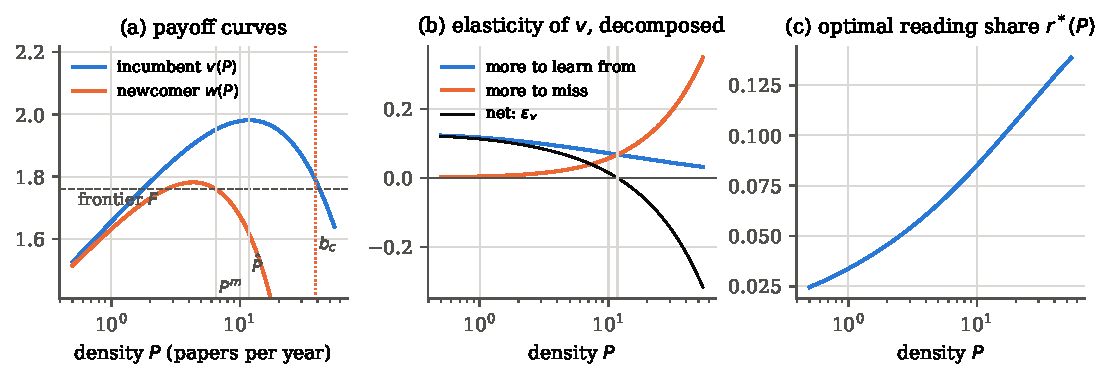
\includegraphics[width=0.98\textwidth]{fig1_payoff_curve.pdf}
\caption{From the paper (its Figure~1). Left: the payoff curve $v(P)$ and the newcomer's payoff $w(P)$ in the calibrated model, with the peak $\Phat$, the mature density $\Pm$ where $w=F$, and the speed limit $b_c$ where $w$ vanishes. Right: the two forces in the slope of $v$ and the optimal reading share.}
\label{fig:payoff}
\end{figure}

\begin{resultbox}{Lemma 5}{Time shares}{\tsolid}
At a given density, $\partial\ln v/\partial\ln b=r^*/(1-r^*)$, and a faster production speed raises the payoff one for one. A speed-up of a task that takes a share $s_k$ of her time saves $s_k\,\dd\ln(\text{speed})$ of her time and raises her payoff by that amount divided by $x^*$. Per unit of time saved, every speed-up is worth the same.
\tcblower
\inwords Inside a topic a tool is worth the time it saves. Reading takes about 7\% of an incumbent's time and production the rest. So a tool that makes reading 30\% faster is worth about 2 log points, and one that makes production 30\% faster is worth 26. Per hour saved they are worth the same.

\why Two lines: the envelope theorem and the first-order condition for reading.

\review Solid, and it does real work: it shows that the old ``writing beats reading'' comparison was mostly about time shares. One caveat: the 7\% comes from a survey of all reading by all faculty and is matched to producing incumbents only. Counting the full-time reading that the model requires of newcomers, reading is 15.8\% of topic members' time (\S\ref{sec:crit-calib}).
\end{resultbox}

\begin{resultbox}{Proposition 1}{The sign of the spillover}{\tsolid}
One more paper in a topic of density $P$ changes each incumbent's payoff by $a\,v'(P)$: positive below the peak, negative above it.
\tcblower
\inwords Whether an extra paper helps or hurts its neighbours is derived, not assumed. It depends on where the topic sits on its payoff curve.
\end{resultbox}

\subsection{Getting into a topic: catch-up}\label{sec:model-catchup}

Careers in a topic end at rate $\rho$, and topics become obsolete at rate $\xi$. The literature a newcomer must master is a stock $S$ that accumulates the flow and loses relevance at rate $\delta$:
\[
\dot S=P-\delta S,\qquad\text{so } S=P/\delta \text{ in a stationary topic.}
\]
She reads it at speed $b_c$ before she can contribute. Papers that appear while she reads must be read too, so her backlog $B$ follows $\dot B=P-\delta B-b_c$ from $B(0)=S$. This is a topic-level version of the ``burden of knowledge'' of Jones (2009).

\begin{resultbox}{Lemma 2}{Catch-up and the speed limit}{\tsolid}
With a constant flow $P$ and an initial stock $S$, catch-up takes
\[
T(P,S)=\frac1\delta\ln\Bigl(1+\frac{\delta S}{b_c-P}\Bigr)\ \text{ if } P<b_c,\qquad T=\infty\ \text{ if } P\ge b_c .
\]
A newcomer to a stationary topic earns on average over her spell
\[
w(P)=v(P)\,\Gamma(P),\qquad \Gamma(P)=e^{-(\rho+\xi)T(P)}=\Bigl(1-\frac{P}{b_c}\Bigr)^{\nu},\qquad \nu=\frac{\rho+\xi}{\delta}.
\]
A share $(1-P/b_c)^{\rho/\delta}$ of a stationary topic's members have caught up and produce.
\tcblower
\inwords Catching up is a race between the reader and the literature. The time it takes rises more than in proportion to the flow, and it is infinite once the literature grows as fast as she reads. Incumbents earn $v$; a newcomer earns $w<v$ because part of her spell goes into reading. Catch-up reading buys admission and nothing else.

\review The formula is right, and it is a real improvement on the linear cost of the previous version. The \emph{limit} it implies depends on an admission standard that incumbents do not meet (\S\ref{sec:crit-speed}). The last sentence, the count of who is producing, is the one that later contradicts Lemma~4 (\S\ref{sec:crit-lemma4}).
\end{resultbox}

\subsection{The frontier}

Instead of joining a topic a researcher can explore. An explorer produces $e$ per period (exploratory work that founds nothing lasting) and founds a viable topic at rate $s$. \emph{A founder stays} in the topic she opens: she wrote its first papers, needs no catch-up, and remains an incumbent until her career there ends or the topic dies. Topics are born at rate $sE$, where $E$ is the number of explorers, and die at rate $\xi$. In a steady state births equal deaths, $sE=\xi M$, where $M$ is the number of open topics.

\begin{resultbox}{Lemma 3}{The value of the frontier}{\tsolid}
The value of exploring per period is
\[
F=(1-\omega)\,e+\omega\,\bar U_F,\qquad \omega=\frac{s}{\rho+\xi+s},
\]
where $\bar U_F$ is the founder's average payoff over the life of the topic she opens. The share of this value that founders earn as incumbents is
\[
\thF=\frac{\omega\,\bar U_F}{F}\in[0,1).
\]
The frontier is depleted as more topics are opened: $F$ falls with the number of open topics at elasticity $\etaF\ge0$.
\tcblower
\inwords Exploring pays in two ways: what you produce while you look, and what you earn as the first insider of the topic you find. $\thF$ is the weight of the second. It is the statistic on which the paper's incidence result turns, and nothing in the paper measures it.

\review The algebra is right. In the stationary economy the paper sets $\bar U_F=v(P)$, as if a newborn topic had its mature density at once. On the paper's own life-cycle simulation founders live mostly through the growth phase and earn 1.82, not 1.95 (\S\ref{sec:crit-founders}). And $\omega$ is the share of time spent as a founder, not a probability as the notation table says.
\end{resultbox}

\begin{resultbox}{Lemma 4}{Output equals the frontier}{\trepair}
In a stationary equilibrium in which every option a free researcher takes is worth $F$, output per researcher is exactly $aF$: \quad $Y=a\,N\,F$.
\tcblower
\inwords If everyone is always indifferent between her options and exploring, then on average everyone earns what exploring is worth. Every question about long-run productivity becomes a question about the frontier.

\why The renewal-reward theorem: a researcher's long-run output per period is the common value of the spells she moves through.

\review This is the step that fails. Its premise does not hold in the economy the paper defines: some members never paid the entry cost. With the member count of Lemma~2, output per researcher is $aF\,e^{\xi T}$, 1.2--3.0\% above $aF$, and the headline numbers change (\S\ref{sec:crit-lemma4}).
\end{resultbox}

\subsection{Equilibrium}

\begin{resultbox}{Definition 1}{Topic equilibrium}{}
A density $P^*$ for every open topic, a production share $x^*$, a number of open topics $M^*$ and a number of explorers $E^*$ such that:
(i)~researchers split their time optimally, $x^*=x^*(P^*)$;
(ii)~newcomers are indifferent between joining and exploring, $w(P^*)=F(M^*,P^*)$;
(iii)~the allocation is stable under entry, $w'(P^*)<0$;
(iv)~births equal deaths and researchers add up, $sE^*=\xi M^*$ and $E^*+M^*n(P^*)=N$.
\tcblower
\inwords Topics fill until joining one is worth no more than opening one. Stability requires that the crossing is on the falling side of the newcomer's payoff: where $w$ still rises, one more entrant makes entry more attractive and draws in more.

The comparative statics are stated in the \emph{large-topic limit}, in which explorers are few relative to topic members, so $M^*\approx N/n(P^*)$.
\end{resultbox}

\begin{keybox}[The model in four sentences]
Inside a topic, more papers first help (more to learn from) and then hurt (more to miss): the payoff curve $v(P)$ has one peak.
Getting into a topic costs reading time that grows with its literature, so newcomers earn $w(P)<v(P)$ and insiders keep the difference.
Outside the topics there is a frontier worth $F$, where people look for new topics and stay in the ones they find.
Topics fill until $w(P^*)=F$.
\end{keybox}

\section{What the model implies}\label{sec:results}

The paper draws its results in four steps: topic choice without an entry cost, topic choice with one, the effect of tools, and what happens to topics over time.

\subsection{Free topic choice without an entry cost}

Set $b_c=\infty$, so newcomers pay nothing to get in and $w=v$.

\begin{resultbox}{Proposition 2}{Equilibrium and dissipation}{\tsolid}
A topic equilibrium exists and is unique. Every open topic sits on the \emph{falling} side of the payoff curve, $P^*>\Phat$. Output per researcher equals the frontier value, $aF<a\vhat$: the gain from cumulative knowledge, $\vhat-F$, is competed away. With founders who stay and no depletion, density solves $v(P^*)=e$ whatever the founders' share.
\tcblower
\inwords A newcomer compares the \emph{average} payoff in a topic with the frontier. She ignores that her papers lower everyone else's payoff once the topic is past its peak. So topics fill past the peak, until being inside is no better than exploring.

\why Crossings on the rising side are unstable: one more entrant raises the payoff of entering.

\review Correct as a benchmark (here Lemma~4 holds exactly). It is the theory of city sizes of Henderson (1974) and of clubs of Buchanan (1965), and the paper says so. What is specific to topics: the hump is derived, the congestion is in attention (``the crowders are the readers''), and the duplication rate depends on density alone. Its implication of equal returns across topics is rejected by Fact~2, which is why the entry cost is added.
\end{resultbox}

\begin{resultbox}{Proposition 3}{Volume opens new topics}{\tsolid}
In the large-topic limit, equilibrium density depends on the number of researchers and on production speed only through the product $Na$, and
\[
\EE\equiv\frac{\dd\ln P^*}{\dd\ln N}=\frac{\etaF}{\etaF D+|\eps_w|+\thF\,\eps_U},\qquad D\ge 1,
\]
where $\eps_w<0$ is the elasticity of the newcomer's payoff with respect to density and $\eps_U$ that of the founder's payoff. New topics absorb a share $1-D\EE$ of growth. If the frontier is not depleted ($\etaF=0$), density, the overlap rate and the aware share do not depend on $N$, on $a$, or on the cost of entering science.
\tcblower
\inwords When the community grows, the extra researchers open new topics until the existing ones are no more attractive than the frontier. Topics get denser only to the extent that good new topics become harder to find. A fixed idea space is the opposite extreme ($\etaF\to\infty$): all growth thickens existing topics.

\role This is where the theory meets the data. Fact~1 measures $\EE$ at 0.12--0.19 against 0.53--0.81 for a fixed idea space. Inverting the formula gives the depletion of the frontier, $\etaF=\EE(|\eps_w|+\thF\eps_U)/(1-\EE D)$. The paper also notes (Remark~4) that mature topics adjust to more researchers \emph{at once}, because the marginal newcomer is indifferent.

\review The algebra is right, and this is the best-supported result in the paper. Two caveats. The formula contains the unmeasured $\thF$, so it should be used to interpret $\EE$, not to derive numbers. And ``only through $Na$'' is a statement about the long run: in the short run more researchers and faster researchers are absorbed very differently, which the paper has in an appendix and which Part~III makes the main idea (\S\ref{sec:ideas-scale}).
\end{resultbox}

\begin{resultbox}{Proposition 4}{Overcrowding and the frontier subsidy}{\trepair}
(i)~Output per researcher at a common density is $a\,w(P)$, so a planner puts every topic at the peak of the newcomer's payoff, $\hat P_w$; she opens more topics with fewer researchers in each. The gain is $\hat w/F-1$.
(ii)~Counting explorers, the planner's density lies between $\hat P_w$ and $P^*$.
(iii)~A subsidy to the frontier (or a tax on joining open topics) of $\hat w-F$ decentralises the optimum.
(iv)~There are two wedges, a \emph{crowding wedge} (newcomers use the average payoff, the planner the marginal one) and a \emph{production wedge} (researchers ignore that their papers add to what colleagues must read). The second vanishes at the optimal density.
\tcblower
\inwords Topics are too crowded and there are too few of them. Fix the allocation of people to topics and the way they split their time takes care of itself.

\review The direction is robust; the size is not. The proof switches between two exponents for the share of members who produce. The planner's gain is 1.25\% under one and 0.37\% under the other, and 0.5--1.0\% once explorers are counted. All are small (\S\ref{sec:crit-lemma4}).
\end{resultbox}

\begin{figure}[h]
\centering
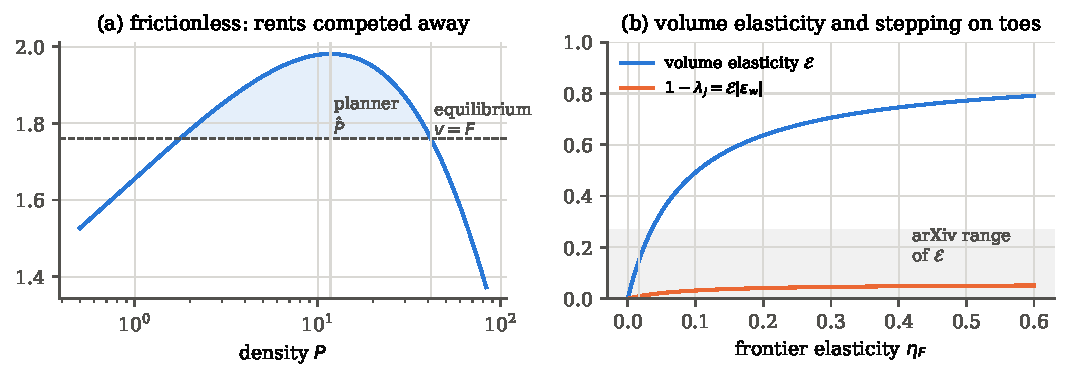
\includegraphics[width=0.98\textwidth]{fig2_planner_volume.pdf}
\caption{From the paper (its Figure~2). Left: without an entry cost topics fill to the density where $v=F$; the shaded rent is competed away and the planner puts topics at the peak. Right: the volume elasticity $\EE$ as a function of the depletion of the frontier; the shaded band is the range of arXiv estimates.}
\end{figure}

\subsection{Topic choice with an entry cost: rents and the speed limit}

Now $b_c<\infty$. Newcomers must read a topic's stock before they contribute.

\begin{resultbox}{Proposition 5}{Mature topics under catch-up costs}{\tsolid}
(i)~The newcomer's payoff $w(P)=v(P)(1-P/b_c)^{\nu}$ has a single peak $\hat P_w$, below the peak of $v$, and vanishes at $b_c$.
(ii)~The mature density $\Pm$ solves $w(\Pm)=F$ on the falling side of $w$. Incumbents earn a premium over the frontier equal to the catch-up cost:
\[
\ln\frac{v(\Pm)}{F}=(\rho+\xi)\,T(\Pm).
\]
(iii)~Mature topics lie on the \emph{rising} side of $v$ when catch-up is costly relative to the rent at the peak.
(iv)~If topics differ in fertility, then across mature topics log returns rise with log density at the catch-up elasticity
$\eps_\Gamma(\Pm)=\nu\,\dfrac{\Pm/b_c}{1-\Pm/b_c}$, which exceeds the premium.
\tcblower
\inwords The entry cost turns the rent that was competed away into a protected one. Insiders earn more than the frontier, by exactly what a newcomer gives up while she reads her way in. More fertile topics attract more people, build larger literatures and protect larger premia. So returns rise with density across topics.

\review Rederived and correct. These results need neither the speed limit, nor the founders' assumption, nor Lemma~4. They are the distinctive, reliable core of the catch-up block. In the calibration the premium is 10.3\% (a catch-up time of 0.74 years) and the gradient is 0.113. The measured gradient (6.7\% per standard deviation) is an upper bound on it, because citations also reward audience.
\end{resultbox}

\begin{resultbox}{Corollary 1}{Overcrowding with rising returns}{\tsolid}
In every stable equilibrium one more member lowers the total output of the others, counting both the spillover on incumbents ($v'$) and the extra reading she imposes on future newcomers ($v\Gamma'$). If $w(\Phat)<F$ then $\hat P_w<\Pm<\Phat$: incumbents' returns \emph{rise} with density ($v'>0$) while the topic is \emph{too crowded} ($w'<0$).
\tcblower
\inwords The data show that the same researcher earns more in denser topics. The natural reading is that topics are too thin. The corollary says that this confuses what an insider earns with what a newcomer can expect. Rising returns are the footprint of an entry barrier, not of an untapped spillover.

\review The sign statement is solid and worth keeping: it is the reason incumbents stay and newcomers go elsewhere. The welfare magnitude attached to it shares the accounting problem of Proposition~4.
\end{resultbox}

\begin{resultbox}{Theorem 2}{The speed limit}{\tinert}
(i)~\emph{Closure.} A topic whose flow is at least $b_c$ is closed: anyone who joins never catches up.
(ii)~\emph{Rents near the limit.} Every mature topic has $\Pm<b_c$. As fertility rises, $\Pm\to b_c$ and both the premium and the returns gradient grow without bound.
(iii)~\emph{Growing topics.} Myopic entry into a growing topic stops before its flow reaches $b_c$.
(iv)~\emph{Production shocks.} A speed-up of production by a factor $1+\alpha$ raises every topic's flow by that factor on impact. Every topic with $\Pm>b_c/(1+\alpha)$ closes and stays closed for at least $\ln[(1+\alpha)\Pm/b_c]/\rho$ periods.
\tcblower
\inwords A literature can grow faster than outsiders can absorb it. When it does, the topic is shut however rewarding it is inside. A tool that lets everyone produce faster pushes the densest topics past the limit for a while.

\review Correct mathematics that never operates. In the calibrated economy the typical mature topic is at 17\% of the limit, the most fertile at 33\%, and no researcher-year is above 53\%. Closing the densest topic needs production to triple. The limit exists only because newcomers must read \emph{everything} while insiders read a third of the flow. Part~(iii) fails with forward-looking entry. A cost with no limit fits the data equally well (\S\ref{sec:crit-speed}). Part~(iv) is the useful piece: it is the seed of the scale-versus-speed idea.
\end{resultbox}

\paragraph{Newborn topics (Remark 6)} A newborn topic has no stock, so its first follower needs no catch-up and earns $v(P_0)$, where $P_0$ is the flow of a newborn topic. New topics attract followers only if $v(P_0)>F$. In the calibration $v(P_0)>F>w(P_0)$: a newborn topic is worth joining while its stock is empty, but a stationary topic of the same density is not. This is the starting point of the life-cycle results below.

\begin{resultbox}{Proposition 6}{Social value and priority transfers}{\tminor}
Part of the credit a duplicate loses is a transfer to the earlier paper. If a share $\tau$ of overlap losses is a transfer, the equilibrium is still overcrowded as long as $\tau<|\eps_w(\Pm)|/(\theta\lambda\Pm)$.
\tcblower
\inwords The welfare results count private credit, and priority credit is partly redistribution. This does not reverse the result, because the reading that newcomers impose on one another is a real cost. In the calibration the critical transfer share is above one. The planner's gain shrinks from 1.2\% to 0.4\% if all overlap losses are transfers.

\review Correct. Not mentioned in the introduction, and nothing else depends on it.
\end{resultbox}

\subsection{Tools}\label{sec:results-tools}

A tool enters the model through one of its parameters: production speed $a$, reading speed $b$, learning $\beta$, search precision $\sigma$, the cost of pivoting $\kappa_p$, catch-up speed $b_c$, or the cost of entering science. Lemma~5 prices each inside a topic. The question of this section is where that value ends up once researchers move.

\begin{resultbox}{Theorem 3}{Frontier incidence}{\trepair}
Let a tool raise the newcomer's payoff $\ln w$ by $h$ and the frontier value $\ln F$ by $f$ at a given density. Then
\begin{gather*}
\dd\ln\frac{Y}{N}=\dd\ln a+\lambda_F\,f+(1-\lambda_F)\,h,\qquad
\dd\ln P^*=\frac{h-f}{\Psi},\\
\lambda_F=\frac{|\eps_w|}{\Psi},\qquad \Psi=|\eps_w|+\thF\,\eps_U+\etaF D .
\end{gather*}
The share of a newcomer-side gain that survives entry is
\[
1-\lambda_F=1-(1-\EE D)\,\frac{|\eps_w|}{|\eps_w|+\thF\,\eps_v}\ \ge\ \EE D .
\]
\tcblower
\inwords In the long run a tool is worth what it adds to the value of opening a new topic. A tool that raises payoffs only inside existing topics draws newcomers in until those topics are again no better than the frontier. Its gain survives only through two channels: founders who stay earn the payoffs of the denser topics they end up in ($\thF$), and fewer topics leave better directions open ($\etaF$). The data put a floor under the surviving share: the volume elasticity.

\review The algebra is right as a statement about the frontier value and about density. The step to output per researcher uses Lemma~4 and fails. Repaired, the theorem has a third channel: members who entered before entry was costly keep their gain too. The numbers move from 14--74\% to 53--88\% (\S\ref{sec:crit-lemma4}). Structurally it is the free-entry incidence result of spatial economics; the application to research tools is new (\S\ref{sec:crit-novelty}).
\end{resultbox}

\begin{resultbox}{Corollary 2}{Ranking tools}{\tassumed}
(i)~\emph{Production tools} act like a larger community: $\dd\ln(Y/N)/\dd\ln a=1-\EE|\eps_w|$, about 0.99.
(ii)~\emph{Learning tools} (reading, learning, search, pivots) raise $v$ at every density. Founders read too, so a share $\Pi_L=1-\lambda_F(1-\thF)$ survives.
(iii)~\emph{Catch-up tools} raise only newcomers' payoffs. Founders never catch up, so a share $\Pi_C=1-\lambda_F$ survives.
(iv)~Hence $\Pi_C\le\Pi_L\le 1-\EE|\eps_w|$.
\tcblower
\inwords Tools that help the people who open topics keep their value. Tools that help only the people who join topics lose most of it.

\review The ordering follows from what explorers are assumed to do: their output scales with production speed and with nothing else, they found topics without reading, and new topics are as fertile as old ones. With the fertility depletion of the paper's own Appendix~B.1 the ranking of production over reading reverses (\S\ref{sec:crit-ranking}). The honest statement is an accounting of where gains go, not a ranking.
\end{resultbox}

\begin{center}\small
\begin{tabularx}{\textwidth}{@{}Lrrrrr@{}}
\toprule
 & \multicolumn{3}{c}{Output per researcher (log points)} & \multicolumn{2}{c}{Footprints ($\omega=\tfrac12$)} \\
\cmidrule(lr){2-4}\cmidrule(l){5-6}
Tool, 30\% better & Fixed topics & Long run, $\omega=0$ & Long run, $\omega=\tfrac12$ & Density & Topics \\
\midrule
Faster production ($a$) & $+26.2$ & $+26.0$ & $+26.0$ & $+3.8$ & $+22.0$ \\
Faster reading ($b$) & $+2.0$ & $+0.3$ & $+1.5$ & $+7.8$ & $-8.0$ \\
Better learning ($\beta$) & $+4.1$ & $+0.5$ & $+2.9$ & $+14.6$ & $-16.3$ \\
Better search ($\sigma$) & $+0.1$ & $+0.0$ & $+0.1$ & $+0.5$ & $-0.4$ \\
Cheaper pivots ($\kappa_p$ halved) & $+0.6$ & $+0.1$ & $+0.5$ & $+2.5$ & $-3.0$ \\
Faster catch-up ($b_c$) & $+2.6$ & $+0.4$ & $+1.0$ & $+26.3$ & $-27.1$ \\
\bottomrule
\end{tabularx}
\par\smallskip
\parbox{\textwidth}{\footnotesize The paper's Table~2, abridged. $\omega$ is the share of an explorer's time spent as the founder of a topic; the paper sets it to one half by assumption. These are the numbers \emph{as the paper reports them}; \S\ref{sec:crit-lemma4} gives the corrected ones.}
\end{center}

\begin{resultbox}{Proposition 7}{Footprints of new research tools}{\tuntested}
(i)~Faster production: density moves with elasticity $\EE$, the number of topics with $1-D\EE$, papers per researcher rise about one for one.
(ii)~Cheaper entry into science raises $N$, with the effects of Proposition~3.
(iii)~Better reading, learning or search, or cheaper pivots: density rises and the number of topics falls. \emph{Science concentrates.}
(iv)~Faster catch-up: the same, more strongly; it also raises the speed limit and makes overshooting more common.
(v)~Better search raises the aware share.
\tcblower
\inwords Each kind of tool leaves a different trace in observables. Reading and catch-up tools pull people into existing topics; production tools do not.

\review Nothing tests it. The only evidence offered, for part~(i), is the ``$+7\%$'' for adopters of language models, which is a pre-existing trend (\S\ref{sec:crit-evidence}).
\end{resultbox}

\begin{resultbox}{Proposition 8}{Valuing output by readership}{\tminor}
Reads per paper are $\mathcal A=(b/a)\,r^*/(1-r^*)$. If output is valued as $\mathcal A^{\alpha}Y$, a production tool adds about nothing at $\alpha=1$ and a reading tool adds about $\dd\ln b$. The ranking of Corollary~2 reverses.
\tcblower
\inwords Total reading is fixed by researchers' time. A faster pen spreads it over more papers, so each paper is read less. A 30\% production tool lowers reads per paper by about a quarter. If science values papers by how much they are read, only reading tools raise output.

\review The reversal is built into the unit: by definition $\mathcal A$ rises one for one with $b$ and falls one for one with $a$. There is no foundation for why doubling reading speed should double the value of science, so the paper reports a ranking and its reversal without a criterion to choose between them. It also omits catch-up reading, which is 29\% of all reads in a mature topic. The thought behind it is the literal meaning of the title, and it deserves a model of its own (\S\ref{sec:ideas-other}).
\end{resultbox}

\subsection{Topics over time, growth and policy}

\begin{resultbox}{Proposition 9}{Too slow and too fast}{\tfragile}
A topic is born with flow $P_0$ and an empty stock, and grows at an exogenous diffusion rate $g$ while entry pays. The stock lags the flow: $S(P)<P/(g+\delta)$.
(i)~\emph{Take-off.} If $w(P_0)<F<v(P_0)$ there is a threshold $g_0$: topics that grow more slowly stall before they are worth joining and are abandoned.
(ii)~\emph{Overshooting.} A topic overshoots the peak of $v$ if and only if $g>g^*=\max\{g_0,g_{\hat P}\}$, with a closed-form bound.
(iii)~\emph{Foresight.} Overshooting survives when newcomers correctly anticipate the topic's path, above a threshold $g^*_{RE}$.
(iv)~\emph{Consolidation.} After entry stops incumbents stay, and the topic thins at rate $\rho$.
\tcblower
\inwords A fast-growing topic has a small literature relative to its current size, so it is cheap to join. People pile in, and the topic ends up larger than is good for it. The reading comes later, for the people who arrive later. A slow topic has the opposite problem: its literature catches up with it before it is big enough to be worth joining.

\review The stock--flow lag is the most original mechanism in the draft. As written it is fragile. Two steps of the proof are verified only numerically (both have short proofs). The take-off threshold exists only for a birth flow between 1.76 and 2.68 papers a year, and 2 is assumed; in the calibration no topic stalls for slow growth. And the law of motion omits the catch-up delay: entrants add to the flow the day they arrive (\S\ref{sec:crit-dynamics}). In the calibration the thresholds are 2.2\% a year for take-off and 20.5\% for overshooting (24.0\% with foresight).
\end{resultbox}

\begin{figure}[h]
\centering
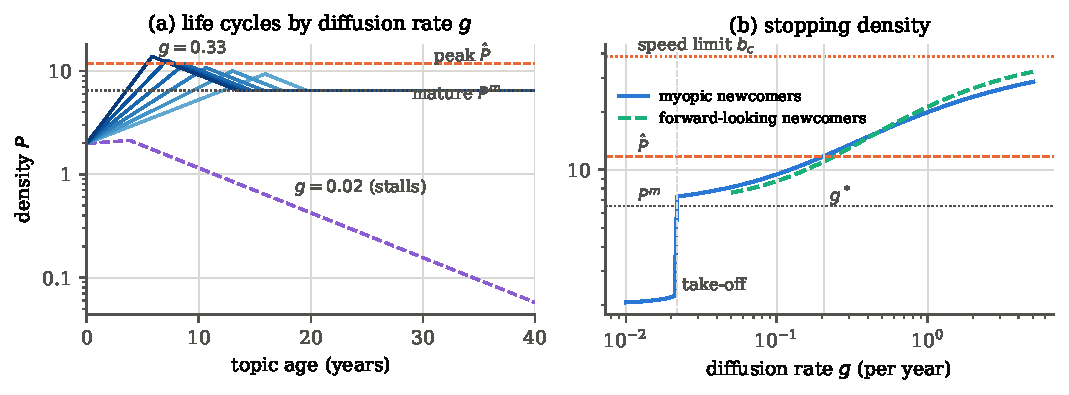
\includegraphics[width=0.98\textwidth]{fig3_lifecycle.pdf}
\caption{From the paper (its Figure~7). Left: density paths of topics with different diffusion rates. A slow topic stalls and is abandoned (dashed); fast ones overshoot the peak and thin slowly. Right: the density at which entry stops, for myopic and forward-looking newcomers.}
\end{figure}

\begin{resultbox}{Proposition 10}{Stepping on toes}{\tfragile}
With $Y=NaF$: \quad $\lambda_J^{\rm eq}=\dd\ln Y/\dd\ln N=1-\EE|\eps_w|$ when topics adjust, and $\lambda_J^{M}=1+\eps_w/D$ when the open topics are held fixed.
\tcblower
\inwords Growth models let ideas scale with researchers as $N^{\lambda_J}$ with $\lambda_J<1$ (``stepping on toes''). Here the parameter is built from two observables. In the calibration it is 0.990 (0.941 with topics fixed): crowding of topics explains little of the measured decline in research productivity.

\review The proof uses Lemma~4, and the number assumes that new topics are as fertile as old ones. With fertility depletion it is an upper bound. It is 0.98--1.00 across every calibration tried, but only because all of them set that depletion to zero.
\end{resultbox}

\begin{resultbox}{Proposition 11}{Policy that depends on a topic's age}{\tfragile}
(i)~A flat subsidy to exploring larger than $v(P_0)-F$ deters the first follower of every newborn topic. No topic then takes off.
(ii)~An entry tax proportional to the stock a newcomer must read is zero in a newborn topic, and with rate $\tau^o=\delta(\hat w-F)/\hat P_w$ it puts mature topics at the peak of $w$.
\tcblower
\inwords The textbook remedy, subsidise the frontier, backfires for young topics: it raises the bar for the people who carry a new topic through its first years. A tax that grows with a topic's literature does not. In practice: reward contributions to young topics more than contributions to old, crowded ones.

\review ``The stationary subsidy (1.25\%) is almost as large as the newborn margin (1.28\%)'' is an artefact of the assumed birth flow and of where the parameter search stopped. Only the ranking survives: the stock tax beats the flat subsidy by a factor of 2 to 5.6, with gains of 0.13--0.72\% of output.
\end{resultbox}

\subsection{The eight extensions of Appendix B}

{\small
\begin{longtable}{@{}P{0.35in}P{1.6in}P{3.75in}@{}}
\toprule
 & Extension & What it shows \\
\midrule
\endhead
\bottomrule
\endfoot
B.1 & Fertility depletion (Proposition 12) & Later topics may be less fertile, at elasticity $\eta_f$. Density data identify only the depletion of \emph{access}, not of fertility. Output per researcher then falls with the number of topics. \textbf{This extension reverses the ranking of tools.} \\
B.2 & Fertility differences & More fertile topics are denser and closer to the speed limit; infertile ones are abandoned. \\
B.3 & Nested topics (Proposition 13) & Topics inside fields give the pattern of Fact~1: close neighbourhoods are pinned, broad ones fill. Two free parameters for two elasticities, so a measurement and not a test. \\
B.4 & Learning from the stock & Stationary results are unchanged. Newborn topics attract followers only if at most 11\% of learning draws on the stock. \\
B.5 & Search on every project (Proposition 14) & If the search for overlap is repeated for every project, production speed no longer drops out of the payoff curve, and faster production lowers search per project. \\
B.6 & Differences in ability & Sorting of able researchers into dense topics could explain part of the returns gradient. Left for future work. \\
B.7 & Credit rules & Only three combinations of the credit parameters matter. \\
B.8 & A production shock over time & Every topic's flow jumps at once, newcomers go to the frontier, topics thin through turnover. \textbf{The seed of the idea in \S\ref{sec:ideas-scale}}, and wrong in two details. \\
\end{longtable}
}

\begin{keybox}[What the theory adds up to]
Without an entry cost, topics fill until nobody gains from being inside (Proposition~2), and growth opens new topics (Proposition~3).
With an entry cost, insiders keep a rent (Proposition~5) and returns rise with crowding in topics that are too crowded (Corollary~1).
A tool is worth the time it saves inside a topic (Lemma~5); after entry, what is left of it is what reaches the frontier (Theorem~3).
Fast-growing topics overshoot because the literature a newcomer must read lags behind (Proposition~9).
\end{keybox}

\section{The evidence, piece by piece}\label{sec:evidence}

The paper has two empirical sections. The first reports five descriptive facts. The second uses arXiv's own rules as sources of variation. This section says what each piece measures and what the paper takes from it. What the review found is in \S\ref{sec:crit-evidence}.

\subsection{The data}

\begin{center}\small
\begin{tabularx}{\textwidth}{@{}P{1.35in}LP{1.3in}@{}}
\toprule
Source & Content & Used for \\
\midrule
An OpenAlex-based panel of arXiv papers & 1.49 million papers posted in 2018--2025, classified into 150 areas by their text; citation counts; a sample of 25,400 full-text PDFs for citing behaviour. \textbf{Not in the repository.} & Facts 1--4 \\
arXiv metadata snapshot of 18 October 2026 & 2.2 million papers from 2015 to 15 October 2026 with the exact time of each submission, the submitter's name, the author list and the abstract. In the repository. & Fact 5 and the six designs \\
INSPIRE-HEP & Curated, complete reference lists and citation counts for high-energy physics. & Validation of awareness; the listing designs \\
\bottomrule
\end{tabularx}
\end{center}

Two measurement devices recur. \emph{Local density} is how many earlier papers lie within a given text-similarity radius of a paper. The \emph{overlap flag} is set when an earlier paper by another group, posted 3 to 24 months before, is closer than the 99th percentile of nearest-neighbour similarity in the paper's area in 2018--19. About 1\% of papers are flagged in the base period; only changes in this rate carry information. Similarity is measured with TF-IDF word weights. The paper notes that TF-IDF and sentence-embedding flags agree on only about a fifth of flagged papers.

\subsection{Five facts}

\subsubsection{Fact 1. Volume opens new ground}
\emph{What is measured.} The elasticity of local density with respect to the volume of papers in the area over the previous two years, with area and year effects.

\emph{What is found.} Between 0.12 and 0.19 at broad radii. If an area's papers kept landing in the same idea space, the same regression would give 0.53 to 0.81 (a benchmark built by randomly thinning each paper's observed list of neighbours). At the radius of the overlap flag the estimate is 0.035 with a standard error of 0.118. In the aggregate, volume rose 122\% between 2018 and 2025 while the overlap rate rose about 13\%.

\emph{How the paper uses it.} It is the volume elasticity $\EE$ of Proposition~3. The paper sets $\EE=0.15$ and reports results over the range from 0 to 0.27. It pins the depletion of the frontier, the floor in Theorem~3 and the stepping-on-toes number.

\subsubsection{Fact 2. Returns are hump-shaped in topic density}
\emph{What is measured.} Citations per author-year for the same researcher in years spent in denser or sparser topics, with author and year effects, on 923,000 author-years. Density is the similarity of a paper to its nearest earlier papers.

\emph{What is found.} One standard deviation of density goes with 6.7\% more citations. Relative to the middle fifth of density, returns are $-11\%$ in the sparsest fifth, $+2\%$ in the fourth and $-2\%$ in the densest. A fitted quadratic peaks about one standard deviation above the mean, with 12\% of researcher-years beyond the peak.

\emph{How the paper uses it.} It rejects the equal returns of the frictionless model and so motivates the entry cost. It supplies five of the eight calibration targets. The paper adds two caveats itself: citations reward audience, so the rising arm overstates the returns to density; and papers per author rise with density ($+0.5\%$ per standard deviation), where Theorem~1(v) predicts a fall.

\subsubsection{Fact 3. Duplicates lose some credit; aware follow-ons gain}
Among flagged papers, those that do \emph{not} cite their nearest earlier paper (unaware overlap) receive 19\% fewer citations than comparable papers; those that do cite it (aware overlap) receive 29\% more. The paper uses these to set the credit parameters $\lambda$ and $\Delta/\lambda$.

\subsubsection{Fact 4. About 60\% of close overlap is aware}
In the PDF sample the later paper cites the earlier one in 35--42\% of flagged pairs. PDF matching recovers 63\% of citations, so the corrected share is about 60\%. Curated reference lists in high-energy physics give 61\% independently. The paper uses the 60\% to set search precision $\sigma$.

\subsubsection{Fact 5. Growth came from new authors; drafting tools raised output modestly}
Papers per author stayed flat while the number of authors grew. In an author-level panel, submitters whose 2023 abstracts adopted the vocabulary that spread with large language models raised their output in 2024--2026 by about 7\% relative to those who did not.

\subsubsection{What the paper withdrew}
A paragraph headed ``What we no longer claim'' retracts two results of an earlier version: that areas with high uptake of language models produced more pioneering papers, and that overlap measured by meaning did not fall. The first used the same TF-IDF neighbours that changes in wording distort; the second has a minimum detectable effect of two thirds of the base rate.

\subsection{Six designs}

\begin{center}\small
\setlength{\tabcolsep}{4pt}
\begin{tabularx}{\textwidth}{@{}P{1.05in}P{2.25in}L@{}}
\toprule
Design & What varies, and what is found & What the paper takes from it \\
\midrule
\textbf{A. Daily cutoff} & A paper submitted just after 14:00 opens the next day's listing. Crossing the cutoff raises the chance of a top-five slot by 0.69 (base 0.30). But the comparison is first against last, submitters differ on the two sides, and top-of-listing papers get \emph{fewer} citations. & Discarded by the authors: it does not isolate visibility. \\
\textbf{B. Rank in the listing} & Position depends on how many other papers happen to be submitted earlier the same day. 87,694 physics papers, 2017--22. One log point lower in the list: citations $-0.023$ (SE 0.016); later unaware overlap by other authors $-0.005$ (SE 0.004) on a mean of 0.068; aware overlap $0.000$. & ``Overlap is detected by targeted search, not by browsing.'' A bounded null. \\
\textbf{C. Endorsement rule} & From 10 December 2025 (Mathematics) and 21 January 2026 (all sections) an institutional e-mail no longer suffices for a first submission. First-time submitters fall by 2.4 points in Mathematics and 3.4 elsewhere, 15--17\% of the base. & A rise in the cost of entering science. The model predicts fewer topics and unchanged density; outcomes need a year of data. \\
\textbf{D. Review rule in computer science} & From 31 October 2025 review and position papers need prior peer review. Their share falls from 2.7\% to 1.3\% (290 to 187 a month). Categories that relied more on reviews saw the first-time-author share fall more ($-0.70$, SE 0.26; placebo a year earlier $-0.32$, SE 0.17). & A rise in the cost of catching up (lower $b_c$). Called ``suggestive''. \\
\textbf{E. Submission cap} & From 1 October 2026 two submissions per person per month. It binds on about 1.3\% of papers. Volume does not fall. & A cap on writing binds on a sliver of output. The paper says it is not a shock to writing speed. \\
\textbf{F. Adopters of language models} & 4,488 of 68,467 submitters used marker words in at least half of their 2023 abstracts. Their output in 2024--26 is higher by 0.022 log points (SE 0.005), ``about 7\%''. & Drafting tools raise output, modestly. \\
\bottomrule
\end{tabularx}
\end{center}

The abstract summarises these as ``four arXiv rule changes and design features identify the margins the model relies on''. The paper is more careful in the body: two of the designs are first stages whose outcomes ``are still accruing'', one reduced form is ``suggestive'', and the catch-up extension ``was added after the returns-by-density evidence was seen, so that evidence cannot test it''.

\subsection{Fifteen predictions}

The paper closes with predictions that were not used to build the model.

\begin{center}\small
\begin{tabularx}{\textwidth}{@{}P{0.3in}LP{0.3in}L@{}}
\toprule
\multicolumn{2}{@{}l}{\emph{Testable with existing data}} & \multicolumn{2}{l}{\emph{Tied to the rule changes or to future tools}} \\
\midrule
P1 & Overcrowding is young and fast: the fall in returns is concentrated where the flow outgrew the stock. & P9 & The blocking of Google in mainland China lowered the aware share there. \\
P2 & Slow clusters die young. & P10 & Endorsement rule: fewer new topics, unchanged density. \\
P3 & Returns follow the stock, density follows the flow. & P11 & Review rule: less entry where reviews mattered. \\
P4 & Newcomers start slowly where stocks are large and flows are fast. & P12 & Submission cap: volume and papers per author unchanged. \\
P5 & The cross-topic gradient is the catch-up elasticity plus audience. & P13 & Reading tools: denser topics, fewer new ones. \\
P6 & Close overlap is pinned; broad neighbourhoods fill. & P14 & A large production shock closes the densest topics to entry. \\
P7 & Founders stay in the clusters they open. & P15 & Better search raises the aware share. \\
P8 & Stepping on toes across areas. & & \\
\bottomrule
\end{tabularx}
\end{center}

\begin{keybox}[What the evidence is, in one sentence]
One fact that bears on a theorem and could have failed (Fact~1); one fact that calibrates (Fact~2); two that calibrate a block the main results do not need (Facts~3 and~4); and six designs that are a discarded discontinuity, a null, two first stages, a non-shock and an estimate that turns out to be a trend.
\end{keybox}

\section{The numbers}\label{sec:numbers}

\subsection{How the model is calibrated}

The model economy is a population of topics, each living through its own life cycle: born thin, growing at its own diffusion rate, maturing, dying. The paper simulates this population, runs on the simulated data the same regressions that produce Fact~2, and chooses parameters to match eight targets.

\begin{center}\small
\begin{tabularx}{\textwidth}{@{}P{2.0in}L@{}}
\toprule
\multicolumn{2}{@{}l}{\emph{Set outside the calibration}} \\
\midrule
Reading and production speed & $b=100$ papers a year, $a=4$ projects a year (normalisations) \\
Credit & $\lambda=0.19$ (Fact 3), detection value $\Delta/\lambda=0.37$, pivot cost $\kappa_p=0.30$ (assumed) \\
Decay of a literature's relevance & $\delta=0.25$ (half-life 2.8 years) \\
Leaving a topic; death of a topic & $\rho=0.10$, $\xi=0.04$ \\
Flow of a newborn topic & $P_0=2$ papers a year (``a few papers per year'') \\
Founding rate & $s=0.14$, chosen so that $\omega=\tfrac12$ \\
\midrule
\multicolumn{2}{@{}l}{\emph{Nine parameters fitted to eight targets}} \\
\midrule
Learning & $\beta=39.5$, $\gamma=0.157$ \\
Erosion per earlier paper & $\theta\lambda=0.0066$ \\
Frontier value & $F=1.760$ \\
Catch-up speed (the speed limit) & $b_c=38.6$ papers a year \\
Search precision & $\sigma=1.61$ \\
Diffusion rate of topics & median 18\% a year, log-sd 0.29 \\
Dispersion of fertility & log-sd 0.043 \\
\midrule
\multicolumn{2}{@{}l}{\emph{Then, from Fact 1 and the frontier equation}} \\
\midrule
Depletion of the frontier & $\etaF=0.0166$, from $\EE=0.15$ \\
Explorers' output & $e=1.70$ \\
\bottomrule
\end{tabularx}
\end{center}

\begin{center}\small
\begin{tabularx}{0.82\textwidth}{@{}Lrr@{}}
\toprule
Target & Data & Model \\
\midrule
Returns gradient per standard deviation of density & 0.067 & 0.052 \\
Sparsest fifth relative to the middle & $-0.110$ & $-0.086$ \\
Fourth fifth relative to the middle & $+0.020$ & $+0.013$ \\
\textbf{Densest fifth relative to the middle} & $\mathbf{-0.020}$ & $\mathbf{+0.022}$ \\
Share of researcher-years beyond the peak & 0.120 & 0.098 \\
Incumbents' premium (an assumed target) & 0.150 & 0.103 \\
Aware share of flagged overlap & 0.60 & 0.61 \\
Reading share of incumbents' time & 0.070 & 0.078 \\
\bottomrule
\end{tabularx}
\par\smallskip
\parbox{0.82\textwidth}{\footnotesize The paper's Table~7. The paper calls the miss on the densest fifth ``the model's main quantitative failure''. It accounts for 12.4 of the total loss of 20.6.}
\end{center}

\subsection{The calibrated economy at a glance}

\begin{center}\small
\begin{tabularx}{\textwidth}{@{}Lr@{\hspace{2em}}Lr@{}}
\toprule
\multicolumn{2}{@{}l}{\emph{A mature topic}} & \multicolumn{2}{l}{\emph{The population}} \\
\midrule
Density $\Pm$ (papers a year) & 6.5 & In-topic researcher-years: growing topics & 24\% \\
Peak of $v$; peak of $w$ & 11.8; 4.3 & \quad in consolidating topics & 20\% \\
Speed limit $b_c$ & 38.6 & \quad in mature topics & 56\% \\
$\Pm$ as a share of the limit & 17\% & Researcher-years beyond the peak of $v$ & 10\% \\
Catch-up time & 0.74 years & Time: writing / catching up / exploring & 76 / 7 / 17\% \\
Incumbents' premium & 10.3\% & Reading share of incumbents' time & 7.3\% \\
Members per topic & 1.9 & Credit lost to overlap & 2.9\% \\
\midrule
\multicolumn{2}{@{}l}{\emph{Slopes at the mature density}} & \multicolumn{2}{l}{\emph{Welfare and growth}} \\
\midrule
Newcomer's payoff $|\eps_w|$ & 0.065 & Planner's gain & 1.2\% \\
Incumbent's payoff $\eps_v$ & $+0.048$ & Stepping on toes (topics adjust) & 0.990 \\
Catch-up $\eps_\Gamma$ & 0.113 & Flat subsidy / stock tax & 0.13 / 0.72\% \\
Volume elasticity $\EE$ (from Fact 1) & 0.15 & Take-off threshold (per year) & 2.2\% \\
Founders' share $\thF$ & 0.55 & Overshooting threshold & 20.5\% \\
\bottomrule
\end{tabularx}
\end{center}

The slope of the newcomer's payoff is worth reading closely. At the mature density it is $-0.065$, made of $+0.082$ from learning, $-0.035$ from overlap and $-0.113$ from catch-up. The force that makes topics crowded for newcomers is the reading they must do to get in. Reading has a third job, admission, and it is the one that carries the model.

\subsection{The headline numbers, as the paper reports them}

\begin{center}\small
\begin{tabularx}{\textwidth}{@{}Lr@{}}
\toprule
Statement & Value \\
\midrule
A 30\% faster producer gains, at fixed topics & 26.2 log points \\
A 30\% faster reader gains, at fixed topics & 1.96 log points \\
Share of a reading gain that survives entry: no founders / founders ($\omega=\tfrac12$) & 14\% / 74\% \\
Share of a catch-up gain that survives: no founders / founders & 16\% / 40\% \\
Share of a production gain that survives & 99\% \\
\textbf{Per hour saved, a production tool is worth \ldots\ times a reading tool} & \textbf{1.3 to 7.2} \\
Valued by readership ($\alpha=1$): 30\% faster production / reading & $+1.3$ / $+21.2$ log points \\
Rent competed away in the frictionless benchmark & 11.2\% \\
Mature topics as a share of the speed limit: typical / most fertile & 17\% / 33\% \\
Production rise needed to close the densest mature topic & threefold \\
\bottomrule
\end{tabularx}
\end{center}

The paper also reports the surviving share on its simulated life cycle, next to the formula of Theorem~3. The two disagree, and Part~II starts from this table.

\begin{center}\small
\begin{tabularx}{0.9\textwidth}{@{}Lrrrrrr@{}}
\toprule
 & \multicolumn{2}{c}{Faster reading} & \multicolumn{2}{c}{Faster catch-up} & \multicolumn{2}{c}{Faster production} \\
\cmidrule(lr){2-3}\cmidrule(lr){4-5}\cmidrule(l){6-7}
Founders' time share $\omega$ & formula & life cycle & formula & life cycle & formula & life cycle \\
\midrule
0 & 17 & \textbf{40} & 17 & 11 & 99 & 99 \\
0.25 & 50 & 44 & 31 & 17 & 99 & 99 \\
0.50 & 74 & 63 & 41 & 17 & 99 & 99 \\
0.75 & 91 & 79 & 48 & 16 & 99 & 99 \\
\bottomrule
\end{tabularx}
\par\smallskip
\parbox{0.9\textwidth}{\footnotesize The paper's Table~9, panel~A: share of the gain at fixed topics that survives entry, in percent. With no founders the formula's 17\% is entirely the depletion of the frontier. The simulation has no depletion and still says 40\%.}
\end{center}

\handoutpart{What holds up and what does not}{This part records every finding of the review. It starts with how the review was done and with what is solid, because a great deal is. It then goes through the problems in order of weight: the structure of the paper, the theory, the numbers, and the evidence. It ends with a scorecard of every result.}

\section{How the review was done}\label{sec:method}

The draft was read five times, independently, each time with one question. The readers, the re-checkers and the reviewers described below were AI agents working from the paper, its code and its data; none of them is a human referee or editor.

\begin{center}\small
\begin{tabularx}{\textwidth}{@{}P{1.1in}L@{}}
\toprule
Reading & Question \\
\midrule
Argument & Read the title, abstract, introduction and conclusion cold. Does the paper reduce to one claim? What would a reader remember after a week? \\
Theory & Is each result correct? Do the results fit together in one economy? What is the smallest set of assumptions each one needs? \\
Evidence & What does each fact and each design identify, and which result does it bear on? Which results have no evidence? \\
Quantification & What does each headline number rest on? What moves if an assumption or the parameter search changes? \\
Referee & A report for a top general-interest journal: novelty against the literature, and the concerns that would decide the outcome. \\
\bottomrule
\end{tabularx}
\end{center}

The theory, evidence and quantification readings were then \emph{re-checked}. A second reader was told to try to refute each finding and to recompute every number from the paper's own code and data. Of the 41 findings re-checked, 29 were confirmed, 12 were confirmed in part and corrected, and none was refuted. The re-checks added nine findings of their own.

Finally, four alternative designs of the paper were written out, each around one central claim, and scored by three reviewers in the roles of a theory editor, an empirical editor and a senior co-author who must decide what to do in the next three months. They too corrected the earlier rounds in two places.

\begin{notebox}[How to read the numbers in Parts II and III]
A number described as \emph{recomputed} was produced from the code in \texttt{code/ftmodel}, from \texttt{code/results/*.json}, or from the data in \texttt{data/} and \texttt{empirics/results/}. Where the first reading and the re-check disagreed, this handout uses the re-check. Judgements, such as the chance of acceptance at a journal, are marked as judgements. Nothing here replaces the authors' own reading of their proofs and data.
\end{notebox}

\section{What is solid}\label{sec:solid}

Before the problems, the things that can be relied on.

\begin{center}\small
\begin{tabularx}{\textwidth}{@{}P{1.75in}L@{}}
\toprule
Result & Why it can be relied on \\
\midrule
\textbf{Theorem 1} (the payoff curve) & The proof was rederived step by step. It needs no functional form. It also does not need the detection block or the time-allocation margin: the hump comes from bounded absorption against a linear risk of being covered. \\
\textbf{Lemma 5} (time shares) & Two lines, correct, and it does real work: inside a topic a tool is worth the time it saves. It replaces the earlier ``writing beats reading by 113 to 1'' with an honest comparison per hour. \\
\textbf{Proposition 5 and Corollary 1} (rents) & The premium equals the catch-up cost; the cross-topic gradient equals the catch-up elasticity; insiders' returns rise with density where the topic is too crowded for newcomers. These hold for any decreasing entry factor $\Gamma$. They need neither the speed limit, nor founders, nor Lemma~4. They are the distinctive core. \\
\textbf{Theorem 3 as algebra} & As a statement about the frontier value and equilibrium density it is right, and it matches re-solved equilibria for small shocks. \\
\textbf{Fact 1, qualitatively} & Every available estimate of the volume elasticity (0.035 at the closest radius, 0.12--0.19 at broad radii, 0.15--0.30 before 2023, 0.19--0.27 in the time series) is far below the benchmark for a fixed idea space (0.53--0.89). \\
\textbf{Three small magnitudes} & Across every calibration tried: the static gain from a better allocation of researchers is 0.15--1.25\% (3.2\% in one variant); credit lost to overlap is 2.9\%; crowding of topics accounts for almost none of ``stepping on toes''. Together these are a finding the paper does not claim: the feared effects are small. \\
\textbf{Data} & 2.2 million timestamped submissions with author lists and text; curated reference lists for high-energy physics; a reconstruction of arXiv's daily listings that is accurate (rank correlation 0.98); two rule changes with sharp, well-timed first stages. \\
\textbf{Code} & It reproduces every number in the paper. All 111 numerical tests of the propositions pass. The problems below are problems of identification, targets and framing, not of implementation. \\
\textbf{Candour} & The draft reports a discarded design, a null with its power, a failed prediction, its main quantitative failure, and two claims it withdrew. \\
\bottomrule
\end{tabularx}
\end{center}

\section{The shape of the problem}\label{sec:crit-structure}

\subsection{Four papers in one}

Read cold, the draft does not reduce to one claim. Each of its outer parts leads with a different one.

\begin{center}\small
\begin{tabularx}{\textwidth}{@{}P{1.2in}L@{}}
\toprule
Where & What it leads with \\
\midrule
Title & The speed limit. \\
Abstract & ``Two results follow'': the speed limit first, then frontier incidence. \\
Introduction & ``Three results organise the paper'': incidence, the speed limit, units. Its first paragraph asks a different question (will faster production flood science with duplicates?). \\
Conclusion & Opens with ``Is innovation too fast?'', a question the introduction never asks, and then calls incidence ``the policy-relevant result''. \\
\bottomrule
\end{tabularx}
\end{center}

\begin{center}\small
\begin{tabularx}{\textwidth}{@{}P{1.55in}P{1.55in}L@{}}
\toprule
Block & Lead results & Standing \\
\midrule
A.\ Topics as cities & Theorem 1, Propositions 2--4, Fact 1 & The only block in which a theorem meets a measured number. No longer in the abstract. \\
B.\ Incidence of tools & Lemmas 4--5, Theorem 3, Corollary 2 & The declared headline. Proof and calibration only. Its key statistic is unmeasured. \\
C.\ Catch-up, speed limit, life cycles & Lemma 2, Theorem 2, Propositions 5, 9, 11 & The title. Proof and calibration only. Nothing in the calibrated economy is near the limit. \\
D.\ arXiv's rules as experiments & Six designs & A discarded discontinuity, a null on a channel outside the model, two first stages, a non-shock, a trend. \\
\bottomrule
\end{tabularx}
\end{center}

Three symptoms follow from this.

\emph{Space is allocated against the argument.} The section that states the declared headline (incidence) has about 1,900 words. The section on arXiv's rules, which does not test it, has about 3,000 and is the longest in the main text. The headline theorem arrives on page 20 of 44, although it needs only two lemmas and ``any payoff curve''.

\emph{The order of sections works against the reader.} The theory uses facts before they are shown (at least twelve forward references). The quantification reports the life-cycle thresholds and the policy gains before the propositions that define them are stated.

\emph{The load is too high for one argument.} Twenty-four named results with about 47 separately lettered claims; an abstract of about 310 words; 47 listed symbols and about 30 unlisted ones, thirteen of them with two or more meanings; each tool reported for six channels, four values of the founders' share, three ways of computing and three units.

\begin{critbox}[The reader's test]
What does a reader remember a week later? In the judgement of the first reading: (1)~output per researcher equals the value of opening a new topic, and inside a topic every hour saved is worth the same; (2)~arXiv doubled while local density barely moved; (3)~insiders' returns rise with density in topics that are already too crowded for newcomers. The speed limit is remembered as a phrase, not a result. ``1.3 to 7.2'' is not remembered, because it has no anchor. The rule changes are remembered as ``data are coming''. None of the three things remembered is what the abstract leads with.
\end{critbox}

\subsection{The evidence tests the previous version}

The two evidence sections were written for version~2, whose questions were overlap, detection, the cost of entry and drafting speed. In the revision that produced version~3 the first of them was not touched and the second changed in one word. The table reads the evidence against the current theory.

\begin{center}\small
\begin{tabularx}{\textwidth}{@{}P{1.3in}P{1.85in}L@{}}
\toprule
Evidence & What it identifies & What it does for the current paper \\
\midrule
Fact 1 & The volume elasticity $\EE$ & \textbf{Tests} Proposition 3, and it could have failed. Gives the floor in Theorem~3. \\
Fact 2 & Returns by density & \textbf{Calibrates} the payoff curve and the catch-up cost (five of eight targets). By the paper's own statement it cannot test the catch-up block. \\
Facts 3 and 4 & Credit of overlapping papers; the aware share & \textbf{Calibrate} the detection block, which the main results do not need. \\
Fact 5; design F & Output of adopters of language models & Nothing: it is a trend (\S\ref{sec:crit-evidence}), and drafting speed is no longer a model object. \\
Design A (cutoff) & --- & Discarded by the authors. \\
Design B (rank) & Whether prominence in the daily listing affects later overlap & A channel that the model does not contain. \\
Design C (endorsement) & Who presses ``submit'' & At most a first stage for the number of researchers. \\
Design D (reviews) & The supply of review articles & A first stage for the catch-up cost, by assumption. \\
Design E (cap) & --- & No model object, in the paper's own words. \\
A 2008 time-use survey & Reading is 7\% of working time & The only source for Lemma~5's numbers. \\
\bottomrule
\end{tabularx}
\end{center}

Read the other way, from results to evidence:

\begin{center}\small
\begin{tabularx}{\textwidth}{@{}P{2.3in}P{0.8in}L@{}}
\toprule
Result & Support & Why \\
\midrule
Proposition 3 (volume opens topics) & Moderate & Fact 1. \\
Theorem 1 (payoff curve) & Weak & The rise in Fact~2; the fall is one fifth, which the model does not match; part~(v) has the wrong sign. \\
Theorem 3 (incidence) & Weak & Only the floor $\EE D$. The founders' share is unmeasured. \\
Lemma 5 (time shares) & Weak & One survey moment. \\
Proposition 10 (stepping on toes) & Weak & Derived from $\EE$ and a model slope. \\
Theorem 2 (speed limit) & None & --- \\
Propositions 8, 9, 11 & None & --- \\
\bottomrule
\end{tabularx}
\end{center}

\begin{critbox}[The first and largest problem]
The current headline rests on four objects: the founders' share $\thF$, the catch-up speed $b_c$, the share of time spent reading, and the indifference of newcomers between topics and the frontier. None of the six designs identifies any of them. The abstract's sentence that the rule changes ``identify the margins the model relies on'' is not supported. An editor who reads the abstract expects evidence on the incidence of tools and on literatures that outrun their readers, and finds evidence on something else.

This is a problem of packaging, not of material: the facts are usable, but they are attached to the wrong claims, and the central claims have no evidence attached.
\end{critbox}

\section{The theory}\label{sec:crit-theory}

The parts of the theory are correct. The centre is not: the paper contains two economies, a stationary one in which the main theorem is stated and a life-cycle one in which everything is quantified, and the first is neither a special case nor a limit of the second. Most of what follows comes from that.

\subsection{The central step: from the frontier value to output}\label{sec:crit-lemma4}

\subsubsection{What goes wrong}
Lemma~4 says that output per researcher equals $aF$. Its premise is that every option a free researcher takes is worth $F$. Lemma~2 gives the count of who is producing: a share $e^{-\rho T}$ of a stationary topic's members. Put the two together. Output per member is $a\,v\,e^{-\rho T}$. Entry makes $v\,e^{-(\rho+\xi)T}=F$. Hence
\[
\text{output per member}=a\,F\,e^{\xi T}\quad\text{and not}\quad aF .
\]
At the calibration ($T=0.74$ years, $\xi=0.04$) the factor is 1.030. Counting explorers, output per researcher is 2.6\% above $aF$ without founders and 1.2\% above with them.

\subsubsection{Why}
The two exponents answer different questions. A newcomer discounts her payoff by $e^{-(\rho+\xi)T}$, because she may leave, \emph{or the topic may die}, before she has caught up. The cross-section count $e^{-\rho T}$ is right only if the members who were there at a topic's birth did not have to catch up. Those members never paid the entry cost. They hold $\xi/(\rho+\xi)=29\%$ of producer-years, and for them ``every option is worth $F$'' is false: they earn more.

So the stationary benchmark mixes two conventions about how a topic is born:

\begin{center}\small
\begin{tabularx}{\textwidth}{@{}P{2.1in}LL@{}}
\toprule
Convention & Used in & Implication \\
\midrule
(a) A topic is born without a stock; its first members are insiders at once & Lemma 2's member count; Remark 6; Proposition 9 & Early cohorts earn rents; output exceeds $aF$ \\
(b) Every member pays the entry cost $T(P)$ & Lemma 4; Theorem 3; the planner's objective & Output equals $aF$ exactly, but young topics are not at the common density \\
\bottomrule
\end{tabularx}
\end{center}

The paper's sentence ``a newborn topic reaches the common density at once'' cannot be made consistent with either: if its first members pay no catch-up they earn more than $F$; if they do, the topic cannot have that flow for its first $T$ years.

\subsubsection{What it does to the numbers}

\begin{figure}[h]
\centering
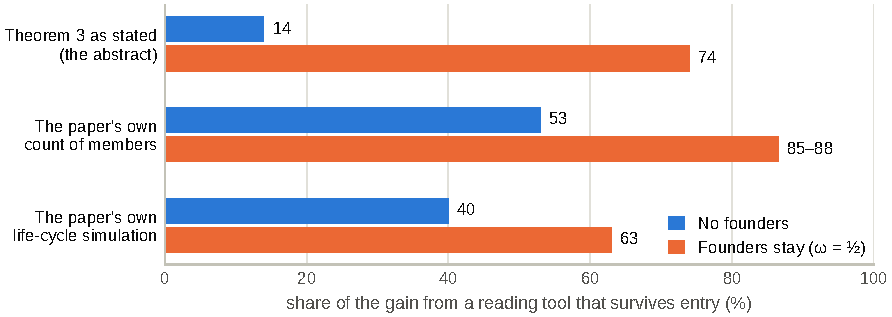
\includegraphics[width=\textwidth]{passthrough.pdf}
\caption{Share of the gain from a 30\% reading tool that survives entry, under three ways of counting. The first is what the abstract reports. The second uses the paper's own count of producing members (Lemma~2) and was obtained by re-solving the equilibrium and measuring output from that count. The third is from the paper's own Table~9.}
\label{fig:passthrough}
\end{figure}

\begin{center}\small
\begin{tabularx}{\textwidth}{@{}Lrrr@{}}
\toprule
 & As stated & Own member count & Own life cycle \\
\midrule
Reading tool, no founders & 14\% & 53\% & 40\% \\
Reading tool, founders ($\omega=\tfrac12$) & 74\% & 85--88\% & 63\% \\
Reading tool, no founders, no depletion & 0\% & 45\% & 40\% \\
Catch-up tool, no founders & 16\% & 25--28\% & 11\% \\
Per hour saved, production over reading & 1.3--7.2 & 1.15--1.9 & 1.25--2.5 \\
\bottomrule
\end{tabularx}
\end{center}

About half of a reading gain survives with no founders at all. The paper's own simulation shows the same thing: with no founders and no depletion the theorem says nothing survives, and the life cycle says 40\%. The paper prints both numbers side by side and leads with the first.

On the life cycle, output per researcher-year is 3.2\% above $F$ without founders. By phase it is $0.99F$ in growing topics (many members still reading), $1.10F$ in consolidating topics (everyone there entered during growth) and $1.04F$ in mature ones (where survivors of the growth phase write 29\% of the papers). All of the excess is the rent of cohorts that entered before entry was costly.

\begin{notebox}
The code never tests Lemma~4. \texttt{equilibrium()} in \texttt{code/ftmodel/equilibrium.py} sets output per researcher to $aF$ by construction, and the test of the incidence formula compares the formula with that. Another test asserts that output per member-year in a mature topic is $F e^{\xi T}$. The two tests pass together because they never meet.
\end{notebox}

\subsubsection{The repair, and why it is an improvement}
The response of the frontier value is correctly characterised by Theorem~3. Only the step from $F$ to output fails, and the fix is one more term:
\[
\dd\ln\frac{Y}{N}=\dd\ln a+\dd\ln F+\frac{\xi}{\rho+\xi}\Bigl(\eps_\Gamma\,\dd\ln P^*-h_\Gamma\Bigr),
\]
where $h_\Gamma$ is the tool's direct effect on the entry factor. For a learning tool the new term adds $\frac{\xi}{\rho+\xi}\,\eps_\Gamma(1-\thF)/\Psi$ to the surviving share: 0.50 without founders or depletion and $0.74+0.13=0.87$ with founders. Exact re-solves give 0.45 and 0.88.

\begin{ideabox}[The economics of the missing term]
Entry \emph{capitalises} a gain that reaches entrants into a higher barrier. A tool that raises the newcomer's payoff by $h$ draws people in until the reading needed to join has grown enough to offset it. The marginal entrant ends up no better off. Insiders do: their payoff rises by $(\eps_\Gamma/|\eps_w|)\,h$, about $1.7h$ at the calibration. A tool's gain therefore stays with whoever is \emph{inframarginal}: the people who open topics, the cohorts that entered before entry was costly, and a scarce frontier. This is a clearer claim than ``output equals the frontier'', and Part~III builds on it.
\end{ideabox}

Three further points belong here.

\emph{The stationary benchmark is not a limit of the life-cycle model.} If topics grow infinitely fast the stock vanishes and they are flooded to just below the speed limit, then thin for about eighteen years. If they grow infinitely slowly they stall. No diffusion rate reproduces the benchmark.

\emph{The planner's gain depends on the convention.} With one exponent the planner's density is 4.3 and the gain 1.25\%; with the other, 5.2 and 0.37\%. Both are smaller than the 3.0\% accounting wedge between the two conventions. The direction (topics are too crowded) is the same under both.

\emph{The paper's Table~9 compares columns that differ in two assumptions.} The ``formula'' column has depletion and values founders at maturity; the ``life cycle'' column has no depletion and puts founders on the simulated path.

\subsection{The founders' channel}\label{sec:crit-founders}

The novelty of version~3 is that founders carry tools to the frontier. Four findings limit it.

\begin{enumerate}
\item \textbf{Founders live through the growth phase.} A founder is present for $1/(\rho+\xi)=7.1$ years. The median topic needs 6.5 years to reach its mature density. So a founder's payoff on the life cycle is 1.82, against 1.95 at maturity and 1.76 at the frontier. On the life cycle the frontier receives 42\% of a reading gain and 1\% of a catch-up gain, against 74\% and 41\% in the stationary formula.
\item \textbf{``Founders stay'' is imposed, not chosen.} In the simulation 36\% of newborn topics attract no follower. Their founders earn less than the frontier value and would do better exploring again.
\item \textbf{Nothing identifies the founders' share.} No calibration moment depends on it. The founding rate is set to 0.14 ``so that half of them found one''. The symbol $\omega$ is the share of an explorer's time spent as a founder, not a probability; the probability of founding is 0.58.
\item \textbf{Varying it changes the economy.} In the life-cycle rows of the paper's table, moving $\omega$ from 0.25 to 0.75 moves the share of researchers who are exploring from 37\% to 6\%. The rows are not a change in founders' incumbency with everything else equal.
\end{enumerate}

\begin{critbox}[The headline range restates two inputs]
With founders, 74\% is the founders' share itself (55 points, from the assumed $\omega=\tfrac12$) plus 18. Without founders, 14\% is $\EE\times D=0.15\times1.11$, evaluated for a 30\% shock. Over $\omega$ from 0 to 0.75 and $\EE$ from 0 to 0.27 the surviving share runs from 0 to 93\%, and the per-hour ratio from 1.06 to 32. The lower end of ``1.3 to 7.2'' is set by an assumption. The upper end is set by the choice of $\EE$, and the paper says that the model's density is the close-radius one, where the estimate is 0.035 with a standard error of 0.118: at that value the ratio is 33, and the ``floor that the data measure'' is statistically zero.
\end{critbox}

\subsection{The ranking of tools is assumed}\label{sec:crit-ranking}

``Production tools survive almost fully; reading tools survive mainly through founders; catch-up tools least'' reads as a result. It is two assumptions.

\textbf{What explorers do.} An explorer ``produces $e$ per unit of production speed''. So the frontier value scales one for one with $a$, and $e$ does not depend on reading speed, learning, search or catch-up. With no founders and no depletion the theorem returns 100\% for production and 0\% for reading by construction; the test suite asserts this as ``full dissipation''. The level of $e$ is a calibrated residual: 1.6--1.8, when a lone researcher in an empty topic earns 1. Exploring is worth 98.8\% of what the best-organised topic pays. All long-run incidence falls on an activity the paper does not model.

\textbf{No fertility depletion.} Appendix~B.1 lets later topics be less fertile, at elasticity $\eta_f$, and shows that density data cannot identify it. Output per researcher then falls with the number of open topics. A reading tool \emph{lowers} the number of topics (by 8 log points; a catch-up tool by 27), so it gains; a production tool raises it and loses.

\begin{center}\small
\begin{tabularx}{0.8\textwidth}{@{}Lrrrrr@{}}
\toprule
Fertility depletion $\eta_f$ & 0 & 0.04 & 0.06 & 0.10 & 0.30 \\
\midrule
Reading tool: share that survives & 13\% & 58\% & 81\% & 126\% & 350\% \\
Production tool: share that survives & 99\% & 96\% & 94\% & 91\% & 74\% \\
\bottomrule
\end{tabularx}
\par\smallskip
\parbox{0.8\textwidth}{\footnotesize Re-solved with the calibrated curves, no founders. Two independent computations put the crossing at $\eta_f\approx0.055$--$0.07$.}
\end{center}

The paper's own growth section says that the measured decline in research productivity ``must come from falling fertility of new topics'' or from selection on ability. If fertility depletion is large enough to matter there, production tools do not ``survive almost fully'', and concentration of science is good, not bad. The caveat appears in Proposition~10 and is absent from Corollary~2 and from the abstract.

\textbf{One technology split in two.} Reading speed is $b=100$ papers a year; catch-up speed is $b_c=38.6$. Nothing relates the two: the first is a normalisation, the second is fitted to rents. A tool that summarises a literature speeds up both, and its incidence lies between the two rows of the paper's table.

\begin{ideabox}[The honest statement]
In the long run a tool is worth the time it saves in the activity of opening topics, plus a term for general equilibrium. Whether production tools or reading tools save more time at the frontier is an empirical question about what the people who open topics do. It can be measured: compare the reference lists and the output of papers that open a new cluster with those of papers that follow.
\end{ideabox}

\subsection{Novelty and positioning}\label{sec:crit-novelty}

In structure the incidence theorem is a known result. Lemma~4 is utility pinned at the outside option, as in the spatial equilibrium of Roback (1982), the migration model of Harris and Todaro (1970), and open-access rent dissipation (Gordon 1954). The formula of Theorem~3 is the two-curve incidence formula: a shift in the newcomer's payoff is divided according to the slope of that payoff and the slope of the frontier. The insiders' premium is the Harris--Todaro queue. There is no land in the model, so local gains are dissipated by congestion and by queueing, not capitalised into rents on land. None of these papers is in the bibliography.

What is new is the application and two features of it: the outside option contains the inside payoff, because founders stay; and tools are classified by whether they move the outside option. A search of the literature found no paper that states the incidence result for research tools. The defensible claim is the application and its measurement, not the theorem.

The speed limit is the stability condition of a queue (delay grows without bound as arrivals approach the service rate), and as economics it is the burden of knowledge of Jones (2009) with the margin of narrowing one's field shut. The take-off and overshooting results are close to models of industry shakeouts and to recent work on research waves. The closest missing references are listed in Appendix~\ref{sec:app-lit}.

\subsection{The speed limit}\label{sec:crit-speed}

\begin{figure}[h]
\centering
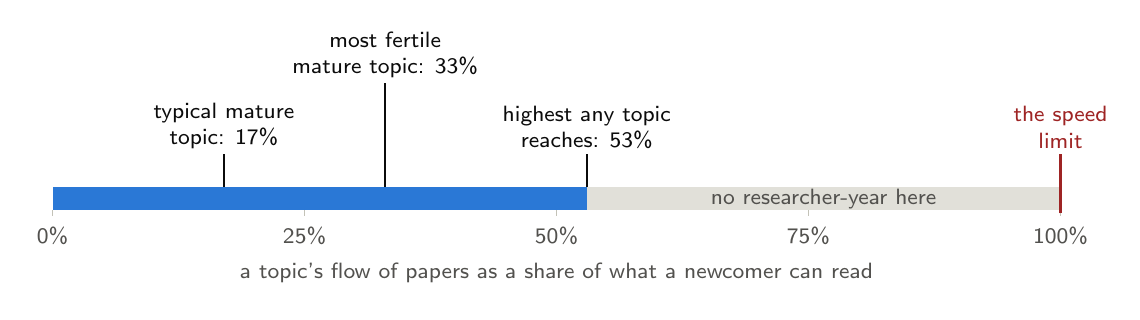
\begin{tikzpicture}[x=0.128cm,y=1cm,font=\sffamily\footnotesize]
\fill[gridc] (0,0) rectangle (100,0.3);
\fill[hblue] (0,0) rectangle (53,0.3);
\foreach \x in {0,25,50,75,100} {\draw[axisc,line width=0.5pt] (\x,-0.07) -- (\x,0); \node[below,color=inktwo] at (\x,-0.08) {\x\%};}
\draw[ink,line width=0.6pt] (17,0.3) -- (17,0.72) node[above,align=center,color=ink,inner sep=1.5pt] {typical mature\\topic: 17\%};
\draw[ink,line width=0.6pt] (33,0.3) -- (33,1.62) node[above,align=center,color=ink,inner sep=1.5pt] {most fertile\\mature topic: 33\%};
\draw[ink,line width=0.6pt] (53,0.3) -- (53,0.72) node[above,align=center,color=ink,inner sep=1.5pt] {highest any topic\\reaches: 53\%};
\draw[stcritdark,line width=1pt] (100,-0.04) -- (100,0.72) node[above,align=center,color=stcritdark,inner sep=1.5pt] {the speed\\limit};
\node[color=inktwo] at (76.5,0.15) {no researcher-year here};
\node[below,color=inktwo] at (50,-0.55) {a topic's flow of papers as a share of what a newcomer can read};
\end{tikzpicture}
\caption{Where the calibrated economy sits relative to the speed limit. Closing the densest mature topic requires production to triple.}
\label{fig:limit}
\end{figure}

Theorem~2 is correct as stated. Six findings say that it should not carry the title.

\begin{enumerate}
\item \textbf{It never operates.} In the simulated cross-section the ratio of a topic's flow to the limit has a median of 0.22, a 99th percentile of 0.39 and a maximum of 0.53. Only 4.6\% of researcher-years are above one third. Closing the densest mature topic needs production speed to rise by a factor of 3.05.
\item \textbf{``17\% of the limit'' is an identity.} In a mature topic $\Pm/b_c=1-\exp(-\text{premium}/\nu)$, and $\nu=(\rho+\xi)/\delta=0.56$ is fixed outside the calibration. With the same premium, a literature that loses relevance twice as fast ($\delta=0.5$) gives 31\%, and four times as fast gives 52\%. The number is the measured spread of returns passed through an assumed ratio of two rates.
\item \textbf{The limit exists because of a double standard.} A newcomer must read the \emph{whole} backlog, at 38.6 papers a year, before she may write anything. An incumbent counts as up to date while reading 7 papers a year at the mature density, 13 at the limit (a third of the flow), and never more than 19. If admission required only what incumbents actually read, no density would be closed.
\item \textbf{Part (iii) holds for myopic entry only.} With forward-looking entry a very fast topic stops above the limit. A figure caption in the paper says the opposite.
\item \textbf{The fit does not need it.} A linear catch-up cost with no limit fits the targets exactly as well (losses of 13.6 and 13.8 after the same search).
\item \textbf{There is no evidence.} The only citation is to a study of attention staying with canonical papers, which is a different mechanism. A referee will ask why the fastest-growing literature of the day has the most entrants.
\end{enumerate}

What survives is the exact catch-up formula, which is better than the linear one, and the convexity of the cost, which matters for how far fast topics overshoot. The limit itself is a remark.

\subsection{Life cycles, take-off and policy}\label{sec:crit-dynamics}

\textbf{The law of motion omits the friction it is about.} In the life-cycle model joiners add to a topic's flow the day they arrive. But a joiner writes only after she has caught up, 0.8 years at the stopping date. People who joined in the last months before entry stops are still reading, and when they start to write the flow keeps rising: by 16\% for the median topic, which carries it past the peak although its growth rate is below the overshooting threshold, and to more than double for a topic growing at 100\% a year, which carries it above the speed limit. The thresholds of Proposition~9 and the statement that entry stops below the limit are properties of a model without a catch-up delay.

\textbf{Two steps of the proof are numerical.} That a stalled topic is abandoned, and that the overshooting threshold equals the stated maximum with the exact stock, are ``verified numerically for the calibrated parameters''. Both have short proofs, which the review wrote out; random searches over parameters found no counterexample.

\textbf{Take-off is a knife-edge that no topic reaches.} The valley in which a slow topic stalls exists only for a birth flow between 1.76 and 2.68 papers a year; the paper assumes 2. In the calibrated population the slowest topic grows at 8.8\% a year, and the take-off threshold is at most 7\% for any topic that can mature. No topic stalls for slow growth. The 36--40\% of newborn topics that fail do so because they are not fertile enough at birth, a margin the paper does not discuss. With forward-looking entry the threshold falls from 2.2\% to 1.0\% a year.

\textbf{The diffusion rate carries the block and is not modelled.} How fast a topic grows rations entry and so generates every rent in the quantification. It is an exogenous random draw, and its distribution is the least well identified part of the calibration.

\textbf{The policy knife-edges are artefacts.}

\begin{center}\small
\begin{tabularx}{0.86\textwidth}{@{}Lrrrrr@{}}
\toprule
Assumed flow of a newborn topic & 1.5 & 1.8 & 2.0 & 2.5 & 3.0 \\
\midrule
Newborn margin $\ln[v(P_0)/F]$ & $-1.7\%$ & $+0.2\%$ & $+1.3\%$ & $+3.4\%$ & $+5.0\%$ \\
Largest share of learning from the stock at which topics are born & 0 & 0.02 & 0.11 & 0.27 & 0.38 \\
Stationary subsidy as a multiple of the margin & --- & --- & 0.97 & 0.37 & 0.25 \\
\bottomrule
\end{tabularx}
\end{center}

``A flat subsidy would bring the economy to the edge of the regime in which new topics attract no followers'' and ``if more than 11\% of learning drew on the stock, no new topic would ever find a follower'' both reverse with a 10\% change in an assumed number. At the better-fitting parameters found by the review (\S\ref{sec:crit-calib}) the newborn margin is 0.1\% and 48\% of topics are stillborn. What survives is the ranking: a tax that rises with a topic's stock beats a flat subsidy by a factor of 2 to 5.6, with gains of 0.13--0.72\% of output.

\subsection{A topic has two members}\label{sec:crit-size}

With the stated normalisation ($a=4$, $b=100$) a mature topic has 1.75 producers and 1.9 members. The planner's best size is 1.15 producers. A newborn topic is half a writer. One more producer raises a topic's flow by 57\% and lowers the newcomer's payoff by 5.4\%, four times the planner's whole gain. More than half of what a member ``learns from'' is her own output.

The density results do not depend on this: with $a=0.4$ a topic has 19 members and every density is unchanged. What does not survive is the language of persons: a first follower, a founder as one insider among many, entry ``one at a time'', diffusion at a continuous rate. The paper must choose between a theory of neighbourhood density (and drop the person-counting) and a rescaling in which a topic is a community of tens.

The same normalisation fixes how much is read. An incumbent reads 7 papers a year, about 20 hours each; a newcomer reads 39 papers a year full time, about 52 hours each. The survey behind the 7\% reading share counts a few hundred article readings a year of about half an hour each. One model ``paper'' is therefore about forty readings, and the paper should say what it is.

\section{The numbers}\label{sec:crit-calib}

The code is clean and reproduces everything, so each of the checks below took minutes. What they show is that the calibration is weaker than the text suggests, and that the numbers the abstract leads with are not the ones the calibration pins down.

\subsection{The reported parameters are not the best fit}

The parameter search runs on a coarse grid and re-ranks its candidates on a fine one. At the reported parameters the two grids disagree (a loss of 17.5 against 20.6). Started from another point, the same model reaches a loss of 13.8 on the paper's own fine grid.

\begin{center}\small
\begin{tabularx}{0.92\textwidth}{@{}Lrr@{}}
\toprule
 & Reported & Better optimum \\
\midrule
Loss on the fine grid & 20.6 & 13.8 \\
Speed limit $b_c$; mature density as a share of it & 38.6; 17\% & 43.2; 16\% \\
Planner's gain & 1.25\% & 1.06\% \\
Slope of the newcomer's payoff & 0.065 & 0.059 \\
Reading pass-through, no founders / founders & 14\% / 74\% & 13\% / 75\% \\
Newborn margin & 1.28\% & 0.10\% \\
Share of newborn topics that attract no follower & 36\% & 48\% \\
\bottomrule
\end{tabularx}
\end{center}

This sorts the paper's numbers by what survives. The incidence numbers, the small planner's gain and the distance from the speed limit survive. The newborn margin and everything built on it do not. The paper's sentence that exact catch-up ``makes the problem harder'' to fit is not supported: all of the apparent worsening relative to the previous version (14.9 to 20.6) is an unfinished search.

\subsection{The model does not reproduce the hump that motivates it}

\begin{figure}[h]
\centering
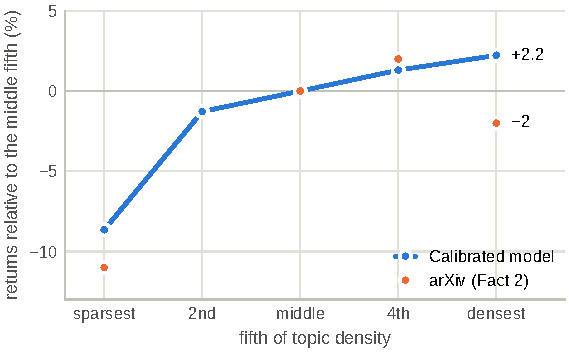
\includegraphics[width=0.66\textwidth]{fit.pdf}
\caption{Returns by fifth of topic density, relative to the middle fifth. In the data the densest fifth earns less than the middle. In the calibrated model returns rise all the way. (The paper does not report the second fifth for the data.)}
\label{fig:fit}
\end{figure}

A single-peaked payoff curve is the paper's founding object, and the hump in returns (Fact~2) is its motivation. In the calibrated model the observable cross-section has no falling arm.

\begin{itemize}
\item Returns are monotone across fifths of density in every parameter vector found. The densest fifth is between $+0.9\%$ and $+2.5\%$ against $-2\%$ in the data. It stays positive when that one moment is given 400 times its weight, and when concurrent overlap is added as a tenth parameter.
\item The paper's fit table compares unlike objects. For the data it reports the peak of a fitted quadratic (one standard deviation above the mean, with 12\% of researcher-years beyond). For the model it reports the peak of the latent payoff curve. Run the same regression on the model's data and the peak is at $+2.67$ standard deviations with 0.001\% of researcher-years beyond it.
\item The reason is structural. Dense topics in the model are the fertile ones, and a mature topic pays its insiders $F/\Gamma(\Pm)$, which \emph{rises} with density (Proposition~5). The cross-section traces the entry condition, not the payoff curve. The remedies the paper suggests (more erosion, concurrent overlap) cannot help.
\item Most of the little curvature the model does show comes from an assumed amount of measurement error in density (a log standard deviation of 0.3) that is hard-coded and not listed as a parameter. Without it the model's cross-section is essentially linear.
\end{itemize}

\begin{ideabox}[What would produce a falling arm]
The cross-topic variation in density would have to come from something that moves the newcomer's payoff but not the insider's: differences across topics in how costly it is to get in. Topics that are easy to enter would then be dense with their rents competed away, and the cross-section would trace the payoff curve itself. This is untested, but it is the natural use of the catch-up block.
\end{ideabox}

\subsection{Identification}

\begin{itemize}
\item \textbf{Nine parameters, eight targets.} One target (an incumbents' premium of 0.15) is assumed, not measured, and is unattainable at the calibrated curve, where the premium cannot exceed 0.119. Five of the eight come from one regression.
\item \textbf{What pins the speed limit.} Not the premium, as the paper's table says, but the share of researcher-years ``beyond the peak'', which is defined differently in the model and in the data, together with the assumed flow of newborn topics.
\item \textbf{What is loose.} The dispersion of diffusion rates is not identified at all. The median diffusion rate, the erosion parameter and the dispersion of fertility are weakly identified. The shares of researcher-years in growing and consolidating topics, and the share that overshoots, inherit this.
\item \textbf{No standard errors.} The loss is not a chi-square statistic. Its scales are tolerances (0.008 for the gradient, against a standard error of 0.0015 in the data).
\end{itemize}

\subsection{The reading share}

The target is 144 hours of article reading a year out of about 2,000, from a survey of all faculty. The model moment counts producing incumbents only (7.8\%). But the model also requires newcomers to read full time while they catch up, and that reading alone is 8.7\% of topic members' time, more than the whole 7\% budget. In total reading is 15.8\% of members' time and 13.2\% of all researcher-years. Either incumbents' reading share should be close to zero, or the catch-up block (a premium of 10\%, nine months of reading) is twice too large for the time-use data.

\subsection{Robust, fragile, artefact}

\begin{center}\small
\begin{tabularx}{\textwidth}{@{}P{1.12in}L@{}}
\toprule
\tsolid & \textbf{Hold across every fit, grid and assumption tried.}
The value of a tool at fixed topics (26.2 and 1.96 log points for 30\% tools; equal per hour).
Production above reading above catch-up, given the frontier assumption.
The planner's gain is small (0.15--1.25\%).
A stock-proportional tax beats a flat subsidy.
The economy is far from the speed limit. \\[4pt]
\tfragile & \textbf{Move with an unmeasured input or across equally good fits.}
14\%/74\% and 1.3--7.2 (0--93\% and 1.1--32 over the plausible range).
The catch-up pass-through (36--69\% across fits; 11--17\% on the life cycle).
The slope of the newcomer's payoff (0.021--0.123), and with it everything that divides by it.
The life-cycle shares (24\% growing, 20\% consolidating, 10\% beyond the peak). \\[4pt]
\tfails & \textbf{Artefacts of an arbitrary choice.}
The newborn margin (1.28\%), the 11\% bound on learning from the stock, ``a flat subsidy about equal to the margin'': the assumed birth flow.
The take-off threshold as a quantitative phenomenon: no topic is below it.
About two members per topic: the normalisation of $a$.
``Peak of $v$ at 0.70 against 1.00 in the data'': different objects.
``Mature topics at 17\% of the limit'': an identity in assumed rates. \\
\bottomrule
\end{tabularx}
\end{center}

\subsection{The stakes}

\begin{critbox}[What the paper can and cannot be about]
Every equilibrium effect in the calibrated model is about 1\% or less: the planner's gain (0.15--1.25\%), the best policy (0.72\%), stepping on toes (0.98--1.00). For reading tools the whole incidence question is whether 0.3 or 1.5 of 2.0 log points survive: a question about 1.2 log points per 30\% tool.

The large numbers are something else. 26.2 against 1.96 is the split of working time, 93\% to 7\%. The reversal under readership units is the same arithmetic in other units. The 11.2\% ``dissipated'' in the frictionless benchmark is a counterfactual the paper itself disowns. The 10\% insiders' premium is distribution, not efficiency.

So this is not a paper about a large distortion. On its own numbers ``innovation too fast'' costs about 1\% of output. It can be a paper about \emph{who gains}, about \emph{where growth lands}, and about two findings stated as such: the static misallocation is small, and crowding explains little of stepping on toes.
\end{critbox}

\section{The evidence}\label{sec:crit-evidence}

\subsection{Fact 1, the anchor}

Fact~1 is the paper's strongest empirical asset: the only evidence that bears on a main result and could have failed. It sets the depletion of the frontier, the floor in the incidence theorem and the stepping-on-toes number. It is not yet at the standard its role requires.

\begin{enumerate}
\item \textbf{The baseline is taken at the wrong radius by the paper's own rule.} The text says that the model's topic is a cell of fixed size, ``so its density is the close-radius density. We therefore use $\EE=0.15$.'' But 0.15 is the middle of the \emph{broad}-radius range. At the close radius the estimate is 0.035 with a standard error of 0.118, an interval from $-0.20$ to $0.27$. The data reject a fixed idea space; they do not pin $\EE$.
\item \textbf{A less favourable estimate is omitted.} The project's own notes report 0.15--0.30 on the years before 2023. The full-sample 0.12--0.19 includes years in which the similarity measure drifted with the wording of abstracts. The paper uses this drift to withdraw its result on pioneering papers, but not to qualify Fact~1.
\item \textbf{The standard errors are the wrong ones.} They are clustered by author, while the regressor varies by area and year across 150 areas. The main range has no standard error at all.
\item \textbf{Attenuation is not discussed.} Only 58\% of a paper's nearest neighbours lie in its own area, which biases the estimate towards zero, the direction that favours the paper. The benchmark is built from the same noisy lists, which handles part of this; by one reader's calculation, 0.15 corresponds to roughly 0.19--0.28 once rescaled by the benchmark.
\item \textbf{Volume is not exogenous.} A new opportunity in an area raises its volume and lowers its local density at the same time. The paper concedes that the inversion ``assumes that the frontier did not move for other reasons''.
\item \textbf{It cannot be reproduced.} The panel behind Facts~1--4 is not in the repository and no script there produces them. The paper says that area clustering ``is part of the replication package''; the project's own notes list it as still open.
\end{enumerate}

The qualitative conclusion very probably survives: even 0.30 is well below 0.53. But the baseline, its interval and its reproducibility have to be repaired before anything is built on it. This is the first gate in Part~III.

\subsection{Fact 2 calibrates; it does not test}

Five of the eight calibration targets come from this one regression. Three points limit what it can carry.

First, ``density'' in the data is a paper's similarity to its nearest earlier papers, not the flow of a topic. Second, citations reward audience, which the paper acknowledges, so the gradient is an upper bound on the returns to density. Third, the one implication of the time-allocation margin that the data can see has the wrong sign. Run on the model's simulated data the way the regression is run on arXiv, papers per researcher fall by 1.3\% per standard deviation of density; in the data they rise by 0.5\% (standard error 0.1). The gap is about a quarter of the whole returns gradient. The paper calls it small.

\subsection{Facts 3 and 4: the credit block}

\begin{enumerate}
\item \textbf{A thin, selected tail.} The $-19\%$ and $+29\%$ compare 3,618 ``unaware'' and 1,381 ``aware'' flagged papers with 468,568 others. Whether a paper cites its nearest neighbour is correlated with its quality and with the prominence of the earlier paper.
\item \textbf{The correction for missed citations is applied to one fact and not the other.} The raw aware share among flagged papers is 27.6\%; corrected for the citations that PDF matching misses, it is about 60\% (Fact~4). So roughly 45\% of the papers called ``unaware'' in Fact~3 do cite the earlier paper. The $-19\%$ is the penalty of a mixed group, and the model's $\lambda$ is taken straight from it. If the misclassified papers earned the aware premium, the penalty for truly unaware duplicates would be far larger.
\item \textbf{At tight radii almost all close pairs share an author.} In high-energy physics the same-author share of later close pairs is 86\% at the 90th percentile of similarity and 95\% at the 99th. The ``other group'' tail on which the flag relies is small and sensitive to how authors are disambiguated.
\item \textbf{An assumed parameter.} The cost of pivoting (0.30) is an assumption, as is the distribution of follow-on credit.
\item \textbf{A contradiction.} Fact~3 says its estimate and the 21\% scooping penalty of Hill and Stein ``validate each other''. The model section says they ``measure different events'': one is duplication of earlier work, the other is losing a race.
\end{enumerate}

The damage is limited, because the main results do not depend on this block. That is also the argument for moving it out of the main text.

\subsection{``Adopters of language models produce 7\% more'' is a trend}

\begin{figure}[h]
\centering
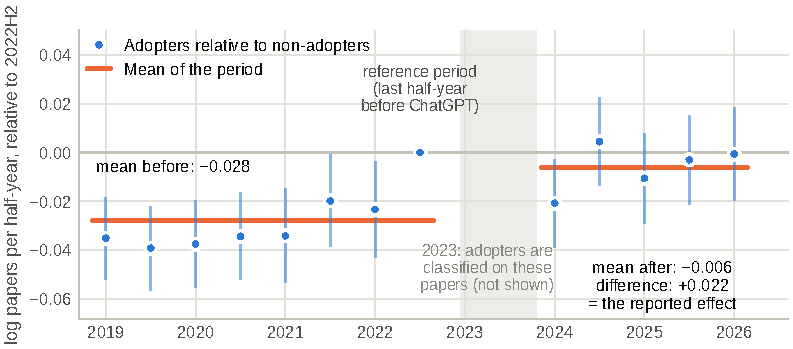
\includegraphics[width=\textwidth]{llm.pdf}
\caption{The paper's own event study, replotted from \texttt{empirics/results/llm\_authors.json}. Output of adopters relative to non-adopters, by half-year, with 95\% intervals; the last half-year before ChatGPT is the reference. The reported effect of 0.022 is the difference between the two orange lines. Relative to the reference period the effect after adoption is zero.}
\label{fig:llm}
\end{figure}

The estimate of 0.022 log points compares the average after 2023 with the average before. But adopters were already catching up with non-adopters before ChatGPT existed: the coefficients rise from $-0.035$ in 2019 to $-0.02$ in 2022. Relative to the last half-year before ChatGPT, the five coefficients after adoption average $-0.006$. A linear trend fitted to the earlier coefficients predicts $+0.010$ for the later window, so against trend the effect is about $-0.016$. The paper says that ``part of this is a pre-existing trend''. All of it is.

The classification is also noisy. Marker words appear in 3.0\% of abstracts in 2022 and 6.6\% in 2023, and 93\% of adopters are classified on one or two flagged abstracts. Adopters already used these words in 6.1\% of their abstracts in 2021--22, against 2.5\% for non-adopters.

This matters in three places: the introduction sets the 7\% against the 36\% of another study; Fact~5 rests on it; and Appendix~B.8 uses it to bound the size of the production shock ``so far'' at ``a few percent''.

\subsection{The designs, one by one}

\begin{center}\small
\begin{tabularx}{\textwidth}{@{}P{1.0in}L@{}}
\toprule
Design & What the review found \\
\midrule
\textbf{Endorsement rule} & The outcome is who presses ``submit''. Re-run on \emph{authors}: in Mathematics the share of papers with a first-time author does not fall ($-0.005$, standard error 0.004, on a base of 0.18), and the staggered contrast is zero ($-0.002$, 0.005). Outside Mathematics new authors per paper fall by about 14\%, with no control group and in the months of the 2026 surge. The paper's sentence that ``the entry margin responds to its cost, which is what makes density respond little to volume'' confuses entry into science with the supply of new topics. The prediction attached to it has no power: the model predicts a change in density of 0.5\% against a minimum detectable effect of two thirds of the base. \\
\textbf{Review rule} & A strong, well-timed first stage ($-1.3$ points, robust to a trend, no leakage). The reduced form on first-time authors ($-0.70$) has a placebo nearly half its size ($-0.32$); the difference is $-0.38$ with a standard error of about 0.31. It is not mechanical ($-0.72$ excluding review-titled papers), but it has no power in counts. The reviews removed are those not accepted by peer review, and reviews still appear after acceptance, so the rule delays more than it removes. Reviews are identified by words in titles, which the rule gives authors a reason to drop. Nothing shows that newcomers used the reviews that disappeared. ``Halved'' describes the share; the count fell by 35\%. \\
\textbf{Listing rank} & A clean design. But its first stage is not significant ($-0.023$ log citations per log position, standard error 0.016), and there are no data on downloads. A zero effect on later overlap is what one would see if detection worked through targeted search, and also if reading did not protect at all. The outcome measures related work, not duplicates. And in the model detection never depends on how prominent the earlier paper was. ``Tight bounds'' and ``detected by targeted search, not by browsing'' go beyond a joint null. \\
\textbf{Submission cap} & No object in the model, as the paper says. The cross-category dose--response is $+0.03$ with a standard error of 2.95, where mechanical removal would give $-1$: it has no content. Fifteen days of data. The sentence that a binding cap ``would be largely dissipated by entry'' contradicts Corollary~2: a cap binds on explorers too and would pass through at about 0.99. \\
\textbf{Daily cutoff} & Correctly discarded by the authors. \\
\bottomrule
\end{tabularx}
\end{center}

\subsection{The fact the paper misses: output per author jumped in 2026}\label{sec:surge}

\begin{figure}[h]
\centering
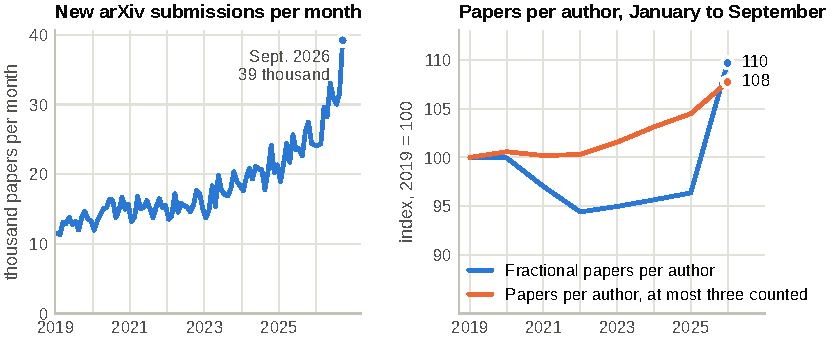
\includegraphics[width=\textwidth]{surge.pdf}
\caption{Computed from \texttt{data/arxiv\_meta.parquet}. Left: new submissions per month. Right: papers per author in January--September of each year, for names with full first names on papers with at most 30 authors. ``Fractional'' gives each author $1/n$ of a paper with $n$ authors.}
\label{fig:surge}
\end{figure}

The paper says that papers per author ``stayed flat'', that growth ``came mostly from new authors'', and that the rise in production so far is ``at most a few percent, too small to produce a visible spike in overlap or to close any topic''. The first two statements are true through 2025. The third is contradicted by the data in the repository.

\begin{center}\small
\begin{tabularx}{\textwidth}{@{}Lrr@{}}
\toprule
January--September & 2025 & 2026 \\
\midrule
Papers & 208,127 & 271,220 ($+30\%$) \\
Papers per submitter (1.47--1.53 in every year 2019--2025) & 1.53 & 1.69 \\
Fractional papers per author (0.50--0.53 in every year 2019--2025) & 0.508 & 0.578 ($+14\%$) \\
\quad the same, authors already active before & 0.580 & 0.658 \\
\quad the same, rare surnames only & 0.444 & 0.497 \\
\quad the same, a fixed cohort active in 2022--24 & 0.556 & 0.634 \\
Share of papers with one author & 10.8\% & 14.8\% \\
Mathematics, papers in September & 3,849 & 8,167 \\
\bottomrule
\end{tabularx}
\end{center}

After seven flat years, output per author rose by 11--14\% in nine months. The rise holds for established authors, for rare names and for fixed cohorts, so it is not a change in who is counted. Of the 30\% growth in volume, between 39\% and 49\% is output per person.

Three cautions belong with the fact.

\begin{itemize}
\item \textbf{It is concentrated among prolific names.} Counting at most three papers per name, the rise is 3.1\% (against 1.3\% the year before); uncapped it is 8.9\% in whole papers. Common names that pool several people inflate this tail.
\item \textbf{It is still building.} Papers per submitter were about 2\% above the previous year in January and February and 6.5\% above in September.
\item \textbf{It is not a pure shock to speed.} The number of authors also rose by about 15\%, three rule changes fall in the same months, and nothing shows what the extra papers are worth.
\end{itemize}

\begin{ideabox}[Why this matters more than any other finding]
Fact~1 was estimated on 2018--2025, years in which output per author was flat. It therefore measures how science absorbs \emph{more researchers}. The paper then uses it to speak about \emph{faster researchers}, which is an extrapolation. The year 2026 is the first time volume grew through output per author. The model says the two kinds of growth land in different places, and for once the data to check a headline claim are already on disk. Part~III builds the recommended paper on this.
\end{ideabox}

\subsection{First data on whether founders stay}

The founders' share is the missing statistic of the incidence theorem. A first cut from data on disk (high-energy physics, 2017--2022) shows that it can be measured, and that the measurement is not straightforward.

Of the later papers that land close to a given paper within two years, 65--70\% share an author with it at a moderate similarity threshold, and 86--96\% at tight ones. But most of this is authors continuing work that nobody else joined. Of 2,476 papers with at least three later close neighbours, 1,046 have no outside author among them. Where at least one outsider follows, the original authors write about 39\% of the later papers; where three or more outsiders follow, about 12\%.

So the founders' share is probably not zero and probably not one half. It is a share of \emph{value}, not of papers; the window is two years; and the radius is a choice. A proper measurement takes two to three weeks (\S\ref{sec:tests}).

\subsection{Statements left over from the previous version}

Eleven statements in the evidence sections contradict the current theory or point to the wrong place. The substantive ones are the ``validate each other'' sentence, the ``faster drafting'' prediction attributed to a proposition about production speed, the cap ``dissipated by entry'', and the attribution of the low volume elasticity to the cost of entering science. The full list is in Appendix~\ref{sec:app-errors}.

\clearpage
\section{Scorecard}\label{sec:scorecard}

Every result, fact, design and headline number of the draft, with the verdict of the review.

\subsection{Theory}

{\small
\begin{longtable}{@{}P{1.55in}P{1.15in}P{3.0in}@{}}
\toprule
Result & Verdict & In one line \\
\midrule
\endhead
\bottomrule
\endfoot
\textbf{Theorem 1} Payoff curve & \tsolid & General and correct. Nearly flat once calibrated; part~(v) has the wrong sign in the data. \\
\textbf{Lemma 5} Time shares & \tsolid & Inside a topic a tool is worth the time it saves. Carry a range for the reading share (7--16\%). \\
\textbf{Proposition 1} Spillover sign & \tsolid & Derived, not assumed. \\
\textbf{Lemma 1} Credit and overlap & \tminor & Correct. Quantitatively inert; the main results do not need it. \\
\textbf{Lemma 2} Catch-up time & \tsolid & The exact formula is right. The limit it implies rests on an admission standard insiders do not meet. \\
\textbf{Lemma 3} Frontier value & \tsolid & Right. The founder's payoff must be taken along her topic's path, not at maturity. \\
\textbf{Lemma 4} Output equals the frontier & \trepair & Contradicts the member count of Lemma~2. Output is $aF e^{\xi T}$; add the rent of early cohorts. \\
\textbf{Proposition 2} Equilibrium, dissipation & \tsolid & The city-size benchmark. \\
\textbf{Proposition 3} Volume opens topics & \tsolid & The best-supported result. A long-run statement. \\
\textbf{Proposition 4} Planner, subsidy & \trepair & Topics are too crowded under every convention; the gain is 0.4--1.25\%. \\
\textbf{Proposition 5} Mature topics, rents & \tsolid & Premium equals the catch-up cost; gradient equals the catch-up elasticity. The distinctive core. \\
\textbf{Corollary 1} Overcrowding with rising returns & \tsolid & The sign statement. Its welfare magnitude shares the problem of Proposition~4. \\
\textbf{Theorem 2} Speed limit & \tinert & Correct mathematics. No researcher-year above 53\% of the limit; a cost without a limit fits as well. \\
\textbf{Proposition 6} Social value & \tminor & Correct. Nothing depends on it. \\
\textbf{Theorem 3} Frontier incidence & \trepair & Right about the frontier value and density. Wrong about output: 53--88\% of a reading gain survives, not 14--74\%. \\
\textbf{Corollary 2} Ranking tools & \tassumed & Follows from what explorers are assumed to do. Reverses with fertility depletion above about 0.06. \\
\textbf{Proposition 7} Footprints & \tuntested & No evidence; the one estimate offered is a trend. \\
\textbf{Proposition 8} Readership units & \tminor & The reversal is built into the unit. \\
\textbf{Proposition 9} Too slow, too fast & \tfragile & The stock--flow lag is original. Two numerical steps; a knife-edge; a law of motion without the catch-up delay. \\
\textbf{Proposition 10} Stepping on toes & \tfragile & Uses Lemma~4 and zero fertility depletion. An upper bound. \\
\textbf{Proposition 11} Policy by age & \tfragile & The knife-edge is an artefact. The ranking of the two instruments survives. \\
\textbf{Proposition 12} Fertility depletion (B.1) & \tsolid & Should be inside the main theorem, where it reverses the ranking. \\
\textbf{Proposition 13} Radius pattern (B.3) & \tminor & Two parameters for two elasticities: a measurement. \\
\textbf{Proposition 14} Search per project (B.5) & \tminor & A qualification of ``production speed drops out''. \\
\textbf{Appendix B.8} A production shock & \trepair & The seed of the main idea. Wrong on how long the excess lasts and on how entry is priced (\S\ref{sec:ideas-scale}). \\
\end{longtable}
}

\subsection{Evidence}

{\small
\begin{longtable}{@{}P{1.55in}P{1.15in}P{3.0in}@{}}
\toprule
Evidence & Verdict & In one line \\
\midrule
\endhead
\bottomrule
\endfoot
\textbf{Fact 1} Volume opens new ground & \trepair & Qualitatively robust. Wrong radius for the baseline, wrong standard errors, an omitted estimate, not reproducible. \\
\textbf{Fact 2} Hump in returns & \tfragile & Calibrates, does not test. The model matches the rise only; one implication has the wrong sign. \\
\textbf{Fact 3} Credit of overlaps & \tfragile & The ``unaware'' group is 45\% misclassified. \\
\textbf{Fact 4} Aware share 60\% & \tsolid & Validated independently in high-energy physics, also at tighter radii. \\
\textbf{Fact 5 and design F} Adopters $+7\%$ & \tfails & Entirely the pre-existing trend. \\
\textbf{Design A} Daily cutoff & \tminor & Discarded by the authors, correctly. \\
\textbf{Design B} Listing rank & \tminor & A clean null on a channel the model does not contain. \\
\textbf{Design C} Endorsement & \tuntested & A first stage on who submits. In Mathematics new authorship does not fall. \\
\textbf{Design D} Review rule & \tuntested & A strong first stage. The reduced form has a placebo nearly half its size. \\
\textbf{Design E} Submission cap & \tminor & No object in the model. \\
\textbf{Not in the paper} The 2026 surge & \tsolid & Papers per author up 11--14\% after seven flat years. The first production shock in the data. \\
\end{longtable}
}

\subsection{Headline numbers}

{\small
\begin{longtable}{@{}P{2.55in}P{1.15in}P{2.0in}@{}}
\toprule
Number & Verdict & Corrected \\
\midrule
\endhead
\bottomrule
\endfoot
A 30\% tool at fixed topics: 26.2 (production) against 1.96 (reading) log points & \tsolid & Equal per hour saved. \\
Reading gain that survives entry: 14\% / 74\% & \tfails & 53\% / 85--88\% with the paper's own count; 40\% / 63\% on its life cycle. \\
Per hour, production is worth 1.3--7.2 times reading & \tfails & About 1.15--2.5; 1.1--32 over the inputs nothing measures. \\
Production gain that survives: 99\% & \tassumed & An upper bound; falls with fertility depletion. \\
Catch-up gain that survives: 16\% / 40\% & \tfragile & 25--28\% without founders; 11--17\% on the life cycle. \\
Mature topics at 17\% (33\%) of the speed limit & \tfails & An identity in assumed rates. \\
Planner's gain 1.2\% & \tsolid & Small in every variant: 0.15--1.25\%. \\
Stepping on toes 0.990 & \tassumed & Holds only with no fertility depletion. \\
Take-off 2.2\%, overshooting 20.5\% a year & \tfragile & No topic stalls; thresholds move with the catch-up delay and with foresight. \\
Flat subsidy 0.13\%, stock tax 0.72\% & \tsolid & The ranking holds (a factor of 2 to 5.6). \\
Newborn margin 1.28\%; ``at most 11\% of learning from the stock'' & \tfails & Artefacts of an assumed birth flow. \\
Readership units: $+1.3$ against $+21.2$ & \tminor & True by definition of the unit. \\
Adopters of language models: $+7\%$ & \tfails & Zero relative to the last period before adoption. \\
``Production shock so far: a few percent'' & \tfails & 11--14\% in January--September 2026. \\
\end{longtable}
}

\handoutpart{Ideas, and what to do}{This part turns the critique into a plan. It states the one idea that the draft contains, develops the two ideas that came out of the review (who keeps the gain from a tool, and the difference between more researchers and faster researchers), compares four ways of writing the paper, and sets out the recommended one with its tests, its fallback and a first month of work.}

\section{The ideas}\label{sec:ideas}

\subsection{One mechanism, four consequences}\label{sec:ideas-one}

The draft has one idea.

\begin{keybox}[The idea]
Entry is the margin on which science adjusts, and the price of entering a topic is reading its literature.
\end{keybox}

\begin{figure}[h]
\centering
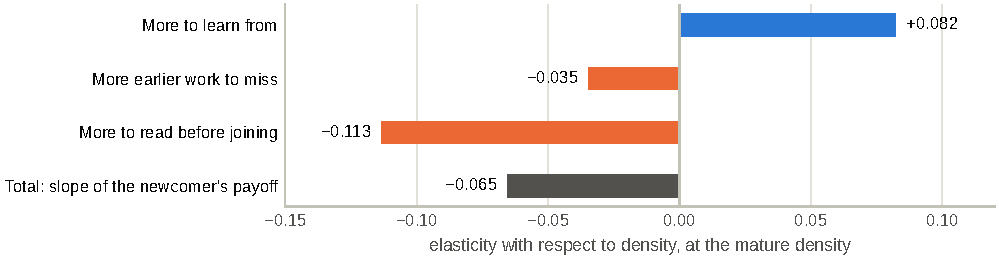
\includegraphics[width=\textwidth]{slope.pdf}
\caption{What makes a topic crowded for a newcomer. The slope of her payoff with respect to density at the calibrated mature density, split into its three parts. Computed from \texttt{code/results/calibration.json}.}
\label{fig:slope}
\end{figure}

Figure~\ref{fig:slope} is the model's own account of it. For someone inside a mature topic, one more paper is good news: the gain from having more to learn from ($+0.082$) exceeds the loss from having more earlier work to miss ($-0.035$). What makes the topic unattractive to someone outside is the reading she must do to get in ($-0.113$). The abstract says that reading has two jobs, to teach and to protect. It has a third, \emph{to admit}, and that is the one that carries the model. The protective job, on which most of the paper's empirical effort is spent, is the smallest of the three.

Four consequences follow from the idea. The draft presents them as separate results.

\begin{center}\small
\begin{tabularx}{\textwidth}{@{}P{1.75in}LP{1.25in}@{}}
\toprule
Consequence & Why it follows & Standing \\
\midrule
\textbf{1. More researchers widen science.} & A free researcher is indifferent between joining a topic and opening one. Extra researchers therefore open topics, and density barely moves. & Evidence in hand (Fact~1), to be repaired. \\
\textbf{2. Insiders earn a rent equal to the entry cost.} & Incumbents have paid; newcomers have not. Returns rise with density even where the topic is too crowded for a newcomer. & Theory solid; the gradient in Fact~2 is consistent with it. \\
\textbf{3. A tool's gain stays with whoever is not on the entry margin.} & The marginal entrant is always indifferent. What she gains is competed away into denser topics and longer reading. & A theorem that needs one repair and one measurement. \\
\textbf{4. Faster researchers are absorbed differently from more researchers.} & New researchers are free and go to the frontier at once. Existing researchers are insiders and stay; when they write more, their topics thicken. & Untested; the data are on disk. \\
\bottomrule
\end{tabularx}
\end{center}

The speed limit is the extreme case of the fourth consequence: a topic whose flow outruns what an outsider can read. Stated as a limit it never binds. Stated as a contrast between two kinds of growth it can be tested this year.

\subsection{Who keeps the gain from a tool}\label{sec:ideas-incidence}

\subsubsection{Three ways of not being on the margin}
The repair of \S\ref{sec:crit-lemma4} changes the incidence result from ``output equals the frontier'' to a statement about who is inframarginal. There are three ways of not being the marginal entrant:

\begin{center}\small
\begin{tabularx}{\textwidth}{@{}P{1.6in}P{1.4in}L@{}}
\toprule
Who & Statistic & Standing \\
\midrule
People who open topics and stay in them & the founders' share $\thF$ & Unmeasured. A first cut suggests it is above zero and below one half. \\
Cohorts that joined before entry was costly & their share of producer-years, $\iota$ (29\% in the stationary count) & Follows from how topics are born; rests on assumed rates of exit and obsolescence. \\
A frontier that is scarce & $\EE D$, from the volume elasticity & Measured, imprecisely. \\
\bottomrule
\end{tabularx}
\end{center}

\begin{ideabox}[A compact form of the repaired result]
For a tool that raises the payoff of everyone inside a topic (reading, learning), the share of the gain that survives entry is
\[
\Pi_L \;=\; 1-\frac{(1-\thF)\,(1-\EE D)\,\bigl[1-\iota\,(1+k)\bigr]}{1+\thF\,k},\qquad k=\frac{\eps_v}{|\eps_w|},
\]
and therefore
\[
\Pi_L\;\ge\;1-(1-\thF)\,(1-\EE D)\,(1-\iota).
\]
\emph{The gain is lost only on researchers who are marginal in all three senses.} The paper's theorem is the special case $\iota=0$, where the floor is $\EE D$.

The formula reproduces the four values established by the review: 0.167 and 0.736 for $\iota=0$ (the paper's numbers before rounding and shock size), and 0.495 and 0.87 with early cohorts. It is a local formula. It has not yet been checked against exact re-solved equilibria over the whole range, and at large $k$ it exceeds one, so it should organise the discussion and not carry a headline number.
\end{ideabox}

\begin{center}\small
\begin{tabularx}{0.9\textwidth}{@{}Lrrrr@{}}
\toprule
 & \multicolumn{4}{c}{Founders' time share $\omega$} \\
\cmidrule(l){2-5}
Volume elasticity $\EE$ & 0 & 0.25 & 0.5 & 0.75 \\
\midrule
\multicolumn{5}{@{}l}{\emph{As the paper states the theorem ($\iota=0$)}} \\
0.035 (the close-radius estimate) & 4\% & 42\% & 70\% & 90\% \\
0.15 (the paper's baseline) & 17\% & 50\% & 74\% & 91\% \\
0.27 (upper end) & 30\% & 58\% & 78\% & 93\% \\
\midrule
\multicolumn{5}{@{}l}{\emph{With early cohorts ($\iota=0.29$, $k=0.73$)}} \\
0.035 & 51\% & 71\% & 85\% & 95\% \\
0.15 & 58\% & 75\% & 87\% & 96\% \\
0.27 & 65\% & 79\% & 89\% & 96\% \\
\bottomrule
\end{tabularx}
\par\smallskip
\parbox{0.9\textwidth}{\footnotesize Share of a small reading gain that survives entry, from the local formula. The upper panel matches the grid recomputed in the review. The lower panel applies the factor $1-\iota(1+k)=0.505$ to the lost share; exact re-solves for 30\% shocks give 53\% and 85--88\% where it gives 58\% and 87\%.}
\end{center}

Two things stand out. With early cohorts, about half of a reading gain survives whatever the frontier and the founders do. And the answer depends much less on the unmeasured founders' share than the paper's range suggests: the band is 51--96\%, not 4--93\%.

\subsubsection{Capitalisation}
The distinctive economic point is what happens to a gain that reaches entrants and not the frontier. Density rises until the reading needed to join has grown enough to offset the gain. The marginal entrant ends up where she started. Insiders gain: for a reading tool, by $(\eps_\Gamma/|\eps_w|)\,h\approx1.7h$, more than one for one. In spatial economics a local improvement is capitalised into the price of land. Science has no land. The gain is capitalised into \emph{the queue to get in}, and it is collected by those who are already inside.

This gives predictions that a shock on the joiners' side could test: after such a shock, density and entry rise, incumbents' returns rise, and the lifetime returns of newcomers do not. No shock with outcomes exists yet; the review rule in computer science is the candidate, and it needs 2027 data.

\subsubsection{An accounting, not a ranking}
\begin{center}\small
\begin{tabularx}{\textwidth}{@{}P{1.5in}LL@{}}
\toprule
Tool & Where its gain goes & What decides the size \\
\midrule
Faster production & To everyone, explorers included, \emph{if} exploring speeds up with production. Lost to the extent that new topics are less fertile. & What explorers do; fertility depletion (unidentified). \\
Faster reading while producing & To insiders at once. After entry: to founders, to early cohorts, and through a scarcer frontier. & $\thF$, $\iota$, $\EE$. \\
Faster catch-up & To entrants at once. After entry: capitalised into denser topics; insiders gain; the frontier gains little. & The slopes $\eps_v$ and $\eps_w$. \\
\bottomrule
\end{tabularx}
\end{center}

What the paper needs here is measurement, not more theory: the founders' share; the share of a topic's output written by people who joined early; what the papers that open topics look like (how much they cite, how much their authors publish) compared with the papers that follow; and a range for the share of time spent reading (7\% to 16\%) carried through every table. With those in hand the nine-parameter calibration can be replaced in the main text by a table of sufficient statistics.

\subsection{More researchers or faster researchers}\label{sec:ideas-scale}

\subsubsection{The observation}
Science can grow in two ways: through more researchers, or through researchers who produce more. Until 2025 arXiv grew in the first way. In 2026 it began to grow in the second (\S\ref{sec:surge}). The paper's long-run result (Proposition~3) says the two are the same thing: density depends on the number of researchers $N$ and on their speed $a$ only through the product $Na$. Its own appendix says that on the way there they are very different, and the difference is a direct consequence of the idea in \S\ref{sec:ideas-one}.

\begin{center}\small
\begin{tabularx}{\textwidth}{@{}P{1.5in}LL@{}}
\toprule
 & More researchers & Faster researchers \\
\midrule
Who are they? & Newcomers, who are free. & Insiders, who have paid the entry cost. \\
Where does the extra output land? & At the frontier, at once: the marginal newcomer is indifferent (Remark~4). & In the topics the insiders are already in: every topic's flow rises at once (Appendix~B.8, Theorem~2(iv)). \\
What happens to density? & Barely moves ($\EE\approx0.15$). & Rises with output per researcher until entry and turnover undo it. \\
Why do insiders not move? & --- & Their payoff rises with density ($v'>0$) and they hold a premium (Proposition~5, Corollary~1). \\
In the long run & \multicolumn{2}{l}{The same: density depends on $Na$ only.} \\
\bottomrule
\end{tabularx}
\end{center}

\subsubsection{What the model predicts for 2026, corrected}

\begin{figure}[h]
\centering
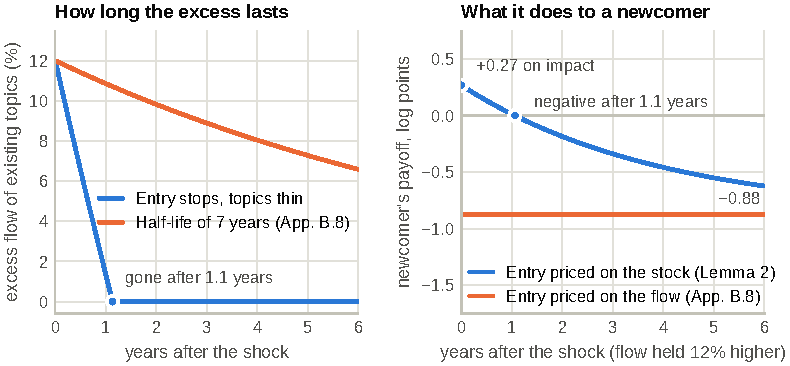
\includegraphics[width=\textwidth]{shock.pdf}
\caption{A production shock of 12\%, the size of the rise in papers per author in 2026, in the calibrated model. Left: the excess flow of existing topics if entry stops and topics thin through turnover, against the half-life stated in Appendix~B.8. Right: the change in a newcomer's payoff when entry is priced on the stock she must read (Lemma~2), against pricing on the flow (Appendix~B.8). Computed from \texttt{code/results/calibration.json}.}
\label{fig:shock}
\end{figure}

The appendix that contains this idea is wrong in two details, and both matter for what the 2026 data can show.

\textbf{How long the excess lasts.} The appendix says the spike decays ``with half-life $\ln2/\rho$'', about seven years. But in the model entry simply stops while topics are too dense, and they thin at the rate $\rho$ at which members leave. A 12\% excess is gone when $1.12\,e^{-\rho t}=1$, after $\ln(1.12)/\rho=1.1$ years. The window in which speed and scale differ is about a year at the assumed rate of exit, and shorter if real turnover is higher.

\textbf{What happens to entry.} The appendix says the newcomer's payoff falls at once. That prices entry on the flow. Lemma~2 prices it on the \emph{stock}, and the stock lags the flow: the day after the shock there is no more to read than the day before, and slightly more to learn from. Her payoff \emph{rises} by 0.27 log points on impact, turns negative after about a year, and ends 0.88 log points lower once the literature has built up.

So the model as written does not predict that entry stops in 2026. Three things follow.

\begin{enumerate}
\item \textbf{Testable now.} Where the extra papers of authors who sped up landed, and whether the flow of existing topics loads more on their incumbents' output than on growth in the number of authors. For a shock that builds up over the year, the reviewers' arithmetic gives a loading of 0.2 to 0.7 if entry stops, 0.9 to 1.0 if it does not respond, against about 0.15 for authors.
\item \textbf{A dated prediction, not a test this year.} Entry into the thickened topics falls in 2027, as their literature builds up.
\item \textbf{Signs, not magnitudes.} Every payoff change behind these predictions is below one log point, and entry in the model is infinitely elastic at indifference. Register the signs and the adding-up of extra flow and lower entry.
\end{enumerate}

\begin{critbox}[Settle the prediction before looking]
Three different predictions for 2026 are on the table: the appendix's (density one for one, a seven-year half-life), the corrected law of motion with entry priced on the flow (the excess absorbed in a year, entry falling at once), and the same with entry priced on the stock (entry unchanged for about a year). Until the authors derive one from a single law of motion, with the stock and the catch-up delay as states, either outcome can be read as support and the test cannot fail.
\end{critbox}

\subsubsection{Three views of the same regression}
The test becomes legible when set against two alternatives.

\begin{center}\small
\begin{tabularx}{\textwidth}{@{}P{2.1in}LL@{}}
\toprule
 & \multicolumn{2}{c}{Response of local density to growth in \ldots} \\
\cmidrule(l){2-3}
View & the number of authors & papers per author \\
\midrule
A fixed idea space & at the benchmark (0.5--0.8) & at the benchmark \\
Free choice of topics, no entry cost (everyone mobile) & low ($\EE$) & low ($\EE$) \\
\textbf{This model} (entry costs reading; insiders stay) & \textbf{low} ($\EE$) & \textbf{high at first, falling to $\EE$} \\
\bottomrule
\end{tabularx}
\end{center}

The first row is rejected by Fact~1. The contrast between the second and third rows is the footprint of the entry cost, and it is what 2026 can show.

\subsubsection{Why this is the natural headline, and its limits}
It is the honest reading of the paper's best fact, which is about scale. It uses the first production shock in the data. It speaks to the question people ask about artificial intelligence: is growth through faster researchers different from growth through more researchers? It needs no founders' share and no calibration for its first half. And it degrades well: if speed turns out to look like scale, the paper keeps a second fact (a rise in output per author did not thicken topics either) and falls back on the entry margin and incidence.

Its limits are real. ``People who write more write near their earlier work'' is what any topic-specific skill predicts; it does not show that the entry cost is \emph{reading}. The stakes inside the model are small. The shock is nine months old, still building, and measured with text similarity in the year in which the wording of abstracts changed. \S\ref{sec:tests} takes these one by one.

\subsection{Other ideas worth keeping}\label{sec:ideas-other}

\begin{enumerate}
\item \textbf{Differences in entry barriers would produce the falling arm.} If topics differ in how costly they are to enter, easy-to-enter topics are dense and their rents are competed away, and the cross-section traces the payoff curve itself (\S\ref{sec:crit-calib}).
\item \textbf{The barrier signature.} Holding a topic's recent flow fixed, a larger stock of older papers should go with fewer newcomers, higher returns for incumbents and no extra exit. A topic that is merely exhausted predicts fewer newcomers, \emph{lower} returns and more exit. Three outcomes, opposite signs. It is the only cheap evidence that the cost of entry is the literature.
\item \textbf{What do the people who open topics do?} Compare the reference lists and the output of papers that open a cluster with those of papers that follow. This turns the ranking of tools from an assumption into a measurement.
\item \textbf{Put fertility depletion inside the theorem} and report results as a function of it, instead of in an appendix that reverses the main corollary.
\item \textbf{Derive the admission standard.} Let a newcomer need coverage $\bar c$ of the stock, which gives a limit of $b_c/\bar c$, and show what survives if the reading required is concave in the stock.
\item \textbf{Add the catch-up delay to the law of motion}, with people who are still reading as a state variable.
\item \textbf{Measure the rates instead of assuming them.} Turnover of authors in topic cells gives $\rho$; the age profile of the references newcomers cite gives $\delta$; cell survival gives $\xi$. The decay rate $\delta$ is the one parameter that could move topics close to the speed limit.
\item \textbf{Entry through apprenticeship.} The model has solo researchers. Much real entry comes with an incumbent co-author, which lowers the reading cost. The share of entry of this kind is measurable.
\item \textbf{Say ``a sunk entry cost'' unless reading is shown.} The results hold for any cost that rises with the stock and that insiders have already paid. The word ``reading'' has to be earned by the stock gradient in item~2.
\item \textbf{State the small magnitudes as findings.} Duplication is pinned by entry, the static misallocation is about 1\%, crowding explains little of stepping on toes. The feared effects are small, and the theory explains why.
\item \textbf{Readership deserves a model.} The literal meaning of the title is that papers are produced faster than they can be read. Proposition~8 only relabels output. A model in which a paper's value comes from being read would make this a result, and it is a different paper.
\item \textbf{Separate rents from sorting.} Able researchers may sort into dense topics. Interacting density with early-career citations distinguishes this from an entry rent.
\item \textbf{Theory of neighbourhoods, not of persons.} State the results for densities and drop ``first follower'' and ``one entrant at a time'', or rescale so that a topic has tens of members.
\item \textbf{A short format.} Two facts, a four-page model, one test. The reviewers judged that this material fits a short paper better than a 40-page model with a calibration.
\end{enumerate}

\section{Four ways to write the paper}\label{sec:designs}

Four designs were written out from the findings of Part~II. Each had to build only on what is solid or can be measured with data on disk, and to add no theory beyond repairs. Three reviewers scored them: one in the role of a theory editor at a top journal, one as an empirical editor, one as a senior co-author who must decide what the team does in the next three months. The ranking was unanimous.

\begin{center}\small
\setlength{\tabcolsep}{4.5pt}
\begin{tabularx}{\textwidth}{@{}L>{\centering\arraybackslash}p{0.45in}>{\centering\arraybackslash}p{0.7in}>{\centering\arraybackslash}p{0.62in}>{\centering\arraybackslash}p{0.72in}>{\centering\arraybackslash}p{0.9in}@{}}
\toprule
Design & One claim & Only solid ground & Evidence in hand & Feasible in three months & Reviewers' odds at a top-5 journal \\
\midrule
\textbf{1. Scale versus speed.} More researchers widen science; faster researchers thicken it first. & 8 & 8 & 5 & 7 & 4--10\% \\
2. The same, plus ``crowding costs about 1\%'' as a second claim. & 6--7 & 6 & 5 & 7 & 3--8\% \\
3. Incidence. Who gains from research tools? & 6 & 6--7 & 3 & 5--6 & 2--6\% \\
4. \emph{Too Fast to Read} as a dynamic paper on catch-up and overshooting. & 5--6 & 4--5 & 1--2 & 3--4 & 1--2\% \\
\bottomrule
\end{tabularx}
\par\smallskip
\parbox{\textwidth}{\footnotesize Scores out of 10, range across the three reviewers. The odds are for the best case. They are judgements, not estimates, and they are the reviewers' own: where the designer of a paper had given a higher figure, the reviewers lowered it.}
\end{center}

\begin{center}\small
\begin{tabularx}{\textwidth}{@{}P{1.0in}LL@{}}
\toprule
Design & Strongest point & Weakest point \\
\midrule
1.\ Scale versus speed & One contrast a reader keeps, built on the two best facts. Its new half can fail in two directions with data on disk. It uses nothing the review refuted, and if the test fails the authors have lost about five weeks. & The robust half of the test (extra papers stay in their authors' topics) is predicted by any topic-specific skill. The discriminating half (entry falls) is not pinned for 2026 and may not be visible until 2027. \\
2.\ With the 1\% claim & The best-ordered plan (two gates) and the clearest table of what each view predicts. & Two claims. The 1\% rests on Lemma~4, on a slope from a regression that cannot be reproduced, and on no fertility depletion. \\
3.\ Incidence & The best economic idea: a gain that reaches only entrants is capitalised into the entry barrier. An honest repair of the central theorem. & The headline cannot fail and cannot be tested before 2027. After the repair it is a band, from a third to nine tenths of two log points, set by inputs that are unmeasured or assumed. \\
4.\ Dynamic & The most original mechanism: the entry cost is a stock, and stocks lag flows. Every object is observable. & No evidence today. Its lead result rests on a law of motion without the catch-up delay. It keeps a title whose object it has to demote. \\
\bottomrule
\end{tabularx}
\end{center}

The five readings of the first round had put incidence first. The three reviewers disagreed, and the reason deserves to be stated plainly. The readings ranked what was in the manuscript, and the 2026 shock was not in it. Incidence is a framework: its statistics are inputs, and nothing in the data can contradict it this year. The contrast between scale and speed is a claim, and the data on disk can reject it.

\section{The recommended paper}\label{sec:recommended}

\subsection{Title, question, thesis}

\begin{keybox}[The paper]
\textbf{Working title.} \emph{More Researchers or Faster Researchers? How Science Absorbs Growth.} To be adopted only if the test supports it.

\textbf{Question.} Does science absorb a rise in output per researcher the way it absorbs a rise in the number of researchers?

\textbf{Thesis.} Newcomers are the margin on which science adjusts, because joining a topic has an entry cost that incumbents have already paid. So more researchers open new topics, while faster researchers first thicken the topics they are already in.
\end{keybox}

\needspace{15\baselineskip}
\subsection{The abstract it could have}

Brackets mark what is not yet established.

\begin{quote}\small
Science can grow through more researchers or through faster ones. The two are absorbed differently. Researchers choose topics, and joining a topic means catching up on its literature. Incumbents have paid that cost and earn a rent, so they stay; newcomers are the margin that adjusts. More researchers therefore open new topics, while faster researchers thicken the topics they are in until entry responds. On arXiv, growth in 2018--2025 came from new authors, and local density rose with an elasticity of [0.12--0.19], against [0.53--0.81] in a fixed idea space. In January--September 2026 papers per author rose 11--14\% after seven flat years. [The extra papers landed in their authors' existing topics, which thickened; new authors again opened new ones.] The model predicts that entry into those topics falls as their literature builds up; we state this as a dated prediction. The welfare effects are small.
\end{quote}

\subsection{The results it would contain}

\begin{center}\small
\begin{tabularx}{\textwidth}{@{}P{0.95in}LP{1.35in}@{}}
\toprule
 & Statement & Comes from \\
\midrule
\textbf{Scale} & More researchers open new topics at once; local density moves with their number at a small elasticity. & Proposition 3, Remark 4, Fact 1 (repaired) \\
\textbf{Speed} & A rise in output per researcher raises the flow of every existing topic. Insiders stay, and the excess is worked off as fast as members turn over. In the long run speed and scale are the same. & Appendix B.8 and Theorem 2(iv), rewritten as one proposition; the 2026 surge \\
\textbf{Why they differ} & Insiders earn a premium equal to the newcomer's entry cost, and their payoff rises with density where the newcomer's falls. & Proposition 5, Corollary 1, Lemma 2 \\
\textbf{The comparison} & If nobody had to pay to get in, speed and scale would be absorbed alike. The asymmetry is the footprint of the entry cost. & A five-line proposition for the frictionless case \\
\textbf{Tools} & Inside a topic a tool is worth the time it saves. A tool that makes researchers faster crowds existing topics first. A tool that makes entry cheaper raises density and insiders' returns. & Lemma 5; the sign statements of \S\ref{sec:ideas-incidence} \\
\bottomrule
\end{tabularx}
\end{center}

The rents are the \emph{mechanism} of the contrast, not a third result. The tools are an \emph{implication}, stated as signs with ranges and no ranking. If either grows back into a headline the paper is several papers again.

\subsection{Outline}

\begin{center}\small
\begin{tabularx}{\textwidth}{@{}P{0.25in}P{1.9in}LP{0.5in}@{}}
\toprule
 & Section & Content & Pages \\
\midrule
1 & Introduction & The question; the two facts side by side; the mechanism in one paragraph; what is and is not claimed. & 3 \\
2 & Two facts & Fact A: the repaired volume elasticity, with its benchmark at every radius. Fact B: the 2026 rise in papers per author. & 5 \\
3 & Model & Topics, the payoff curve (stated; proof in the appendix), the exact catch-up cost, the frontier value, equilibrium. Fewer than 20 symbols. & 5 \\
4 & Scale and speed in the model & The five results above. & 5 \\
5 & The 2026 test & Measurement; where extra papers land; crowding and entry; threats. & 8 \\
6 & What this means for research tools & Lemma 5 and the two sign statements. & 2 \\
7 & Magnitudes & The two elasticities, turnover, adjustment time; the small numbers as findings. & 2 \\
8 & Conclusion & The dated predictions for 2027. & 1 \\
\midrule
 & Appendices & Proofs; data and name keys; robustness; the rule changes as context; the calibration as an illustration. & \\
\bottomrule
\end{tabularx}
\end{center}

About thirty pages. The reviewers' advice was to aim lower still.

\subsection{What goes where}

\begin{center}\small
\begin{tabularx}{\textwidth}{@{}LP{2.2in}@{}}
\toprule
Material in the current draft & Place \\
\midrule
Proposition 3, Remark 4, Fact 1 & Lead: scale \\
Appendix B.8, Theorem 2(iv), the 2026 surge & Lead: speed \\
Proposition 5, Corollary 1 (signs), Lemma 2 without the label ``speed limit'' & The mechanism \\
Lemma 5; the repaired output accounting & A short section on tools \\
Theorem 3 with the inframarginal term; the founders' share & The fallback, or a second paper \\
Theorem 1; the calibration; Propositions 4 and 10 as ranges & Appendix, plus a paragraph of magnitudes \\
Theorem 2(i)--(iii); Propositions 9 and 11; the life-cycle simulation & Shelved, for a paper with its own evidence \\
Lemma 1; Facts 3--5; the listing designs; the cap; Propositions 6 and 8 & Out, or a data appendix \\
Fact 2 & Kept only as an upper bound on the catch-up gradient \\
Fifteen predictions & Three or four, about the path in 2027 \\
``What we no longer claim''; every sentence about earlier versions & Deleted \\
\bottomrule
\end{tabularx}
\end{center}

\section{The tests}\label{sec:tests}

\subsection{Two facts}

\textbf{Fact A (scale).} Repair Fact~1 on its own panel: standard errors clustered by area or by wild bootstrap, every radius next to its benchmark, the years before 2023, embedding-based neighbours. Then build a version that runs from the repository: arXiv's primary categories, density measured as a flow (neighbours posted in the previous twelve months), regressed on the number of authors and on papers per author separately. Both elasticities of the paper must come from one panel and one measure.

\textbf{Fact B (speed).} Write up the 2026 rise by field and by month, with authors and not submitters, for a fixed cohort, with papers per name capped at three, five and ten, with and without catch-all categories. This needs no text measure and can be done first.

\subsection{Three tests}

\begin{center}\small
\begin{tabularx}{\textwidth}{@{}P{1.05in}LL@{}}
\toprule
Test & Construction & What supports, what refutes \\
\midrule
\textbf{A. Where do the extra papers land?} & A fixed cohort of author names active in each of 2022--2024. For each of their papers: is it in a topic cell where the author published before? Is its category one of the author's earlier categories (a version that uses no text)? How many papers by others lie nearby? Regress on the author's change in output, with author effects and category-by-year effects. Placebo: the change from 2024 to 2025. & \emph{Supports:} authors who sped up keep the same share of papers in their home cells, and the extra papers sit in cells at least as dense. \emph{Refutes:} the extra papers land outside home cells, in thin or new ones. Then speed behaves like scale. \\
\textbf{B. Do their topics thicken, and does entry respond?} & Topic cells fixed on 2022--24 text, at three sizes chosen in advance. Split each cell's flow into papers by incumbents, by movers (already on arXiv, new to the cell) and by first-time authors. The cell's speed shock is the change in its incumbents' output \emph{outside} the cell, so that an opportunity specific to the cell does not drive it. Regress the change in the cell's flow on the speed shock and on growth in authors; regress movers' entry on the speed shock. & \emph{Supports:} the flow loads on the speed shock clearly more than on growth in authors. \emph{Half a result:} flow up, entry unchanged; the fall in entry is then the dated prediction. \emph{Refutes:} speed and scale load alike. \\
\textbf{C. Two elasticities in one regression} & Categories by half-year, 2019--2026: local density on the number of authors and on papers per author. & A consistency check only. Across categories the rise in papers per author has a standard deviation of 0.04, about 0.03 of it signal, so the standard error is near 0.3. \\
\bottomrule
\end{tabularx}
\end{center}

The cell-level and author-level tests carry the paper. The cohort is large (of the order of 100,000 names), which is where the power is.

\subsection{Threats, and what answers them}

\begin{center}\small
\begin{tabularx}{\textwidth}{@{}P{1.45in}L@{}}
\toprule
Threat & Defence \\
\midrule
\textbf{The wording of abstracts changed in 2025--26.} Word-based similarity fell; embedding-based similarity may err the other way, and the authors who sped up may be the ones whose wording changed. & Comparisons within a category and period. Versions that use no text: the author's home category; cells built from shared references in high-energy physics. A ``style floor'': the similarity of random pairs across categories in each half-year, with radii defined relative to it. A subsample of abstracts rewritten by one fixed procedure before embedding. \\
\textbf{Three rule changes in the same months.} & Count authors, never submitters. Define displaced entrants as authors already on arXiv, on whom the endorsement rule does not bind. Drop review-titled papers. Make mathematics and physics the main sample. End the window on 30 September, before the cap. \\
\textbf{The extra papers may be of low quality.} If newcomers ignore them, they add nothing to what must be read. & A fixed cohort of established authors. Drop catch-all categories and withdrawn papers. In high-energy physics, split the extra papers by early citations. This is the hardest threat: early citations are thin. \\
\textbf{The rise is concentrated among prolific names.} & Caps at three, five and ten papers per name; rare surnames; names above the 99th percentile trimmed. \\
\textbf{A common shock raises output and density together.} & The leave-out construction of the speed shock. Flat pre-trends in 2024--25. A lead test: the size of a cell's 2026 shock must not predict its change in 2024--25. \\
\textbf{The result is read after the fact.} & A dated memo, deposited before any 2026 similarity is computed: outcomes, samples, radii fixed on 2019--22, cells fixed on 2022--24, thresholds for ``supports'' and ``refutes'', and a power calculation on the placebo years. \\
\bottomrule
\end{tabularx}
\end{center}

\subsection{Is the entry cost the literature?}

None of the three tests shows that the cost of entry is \emph{reading}. Two by-products of the same panel bear on it. First, measured turnover: the share of a cell's papers written by authors new to it, by year, which replaces the assumed rate of exit and gives the adjustment time. Second, the barrier signature of \S\ref{sec:ideas-other}: holding a cell's recent flow fixed, does the newcomers' share fall with the stock of older papers, while incumbents' returns rise and their exit does not? If the stock gradient is absent, the paper says ``a sunk entry cost'' and keeps Lemma~2 as its leading example.

\needspace{12.5cm}
\subsection{Two gates}

\begin{figure}[h]
\centering
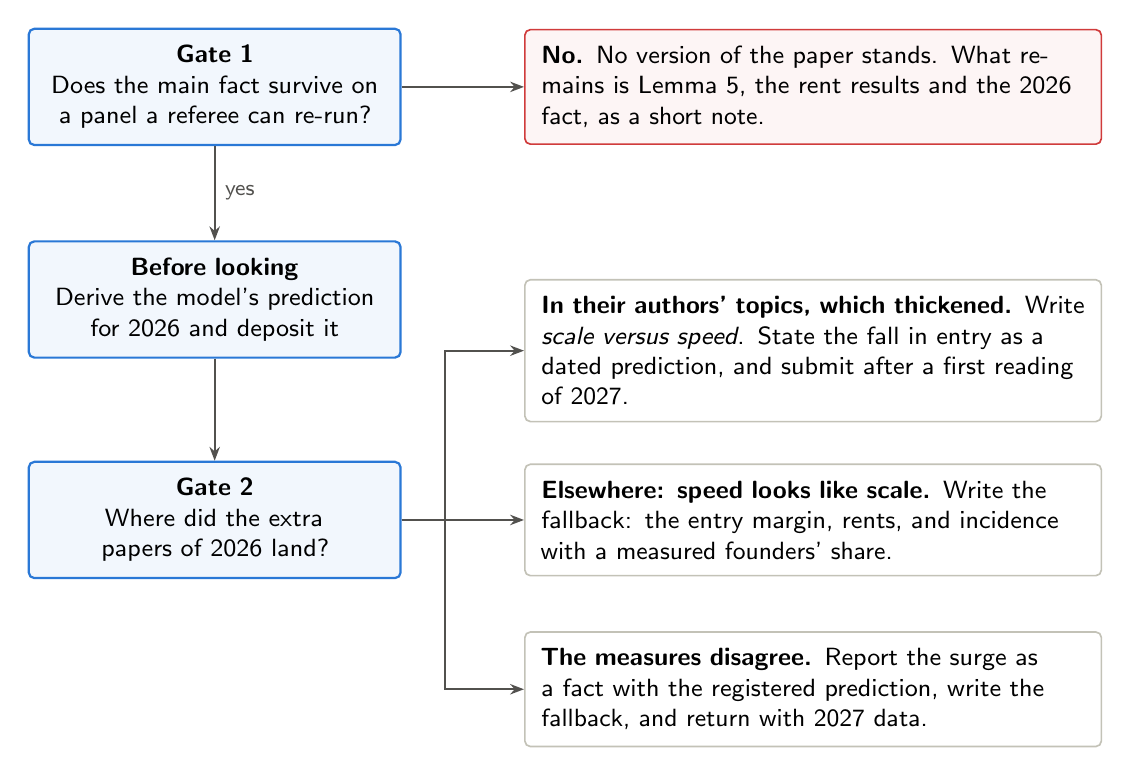
\begin{tikzpicture}[font=\sffamily\small,
 gate/.style={draw=hblue,line width=0.8pt,rounded corners=2pt,fill=hblue!6,align=center,inner sep=6pt,text width=4.3cm},
 outc/.style={draw=axisc,line width=0.6pt,rounded corners=2pt,fill=white,align=left,inner sep=6pt,text width=6.9cm},
 stopc/.style={outc,draw=stcrit,fill=stcrit!5},
 arr/.style={-{Stealth[length=5pt]},line width=0.8pt,color=inktwo},
 lab/.style={font=\sffamily\footnotesize,color=inktwo}]
\node[gate] (g1) at (0,0) {\textbf{Gate 1}\\Does the main fact survive on a panel a referee can re-run?};
\node[gate] (pre) at (0,-2.7) {\textbf{Before looking}\\Derive the model's prediction for 2026 and deposit it};
\node[gate] (g2) at (0,-5.5) {\textbf{Gate 2}\\Where did the extra papers of 2026 land?};
\node[stopc] (s1) at (7.6,0) {\textbf{No.} No version of the paper stands. What remains is Lemma~5, the rent results and the 2026 fact, as a short note.};
\node[outc] (o1) at (7.6,-3.35) {\textbf{In their authors' topics, which thickened.} Write \emph{scale versus speed}. State the fall in entry as a dated prediction, and submit after a first reading of 2027.};
\node[outc] (o2) at (7.6,-5.5) {\textbf{Elsewhere: speed looks like scale.} Write the fallback: the entry margin, rents, and incidence with a measured founders' share.};
\node[outc] (o3) at (7.6,-7.65) {\textbf{The measures disagree.} Report the surge as a fact with the registered prediction, write the fallback, and return with 2027 data.};
\draw[arr] (g1) -- node[lab,right] {yes} (pre);
\draw[arr] (pre) -- (g2);
\draw[arr] (g1) -- (s1);
\draw[arr] (g2.east) -- ++(0.55,0) |- (o1.west);
\draw[arr] (g2.east) -- (o2.west);
\draw[arr] (g2.east) -- ++(0.55,0) |- (o3.west);
\end{tikzpicture}
\caption{The order of decisions. The first month of work is the same under every outcome, so nothing is lost by choosing the headline at the end of it.}
\label{fig:gates}
\end{figure}

\subsection{The fallback and the second paper}

\textbf{The fallback.} If speed looks like scale, incumbents are mobile at the margin, and every result that needs members to stay put is rejected with it (Appendix~B.8, Theorem~2, Proposition~9). The paper is then the one the first round agreed on: the entry margin (Proposition~3 and Fact~1, with a second fact that a rise in output per author did not thicken topics either), rents as the reading of the returns gradient, and the incidence of tools with sufficient statistics. That paper needs the founders' share.

\textbf{Measuring the founders' share.} In high-energy physics, where reference lists are complete: call a paper a \emph{pioneer} if no earlier paper lies within a fixed radius in the previous 24 months, and its cell \emph{founded} if at least a given number of later papers by other authors land in it. For the authors of pioneers, split their citation-weighted output over the next five years into work in cells they founded and that drew followers, work in cells founded by others, and work that nobody followed. The founders' share is roughly the first as a fraction of the first and the third. Two to three weeks. The radius is the risk: fix it and the thresholds in the dated memo, and report across radii. The same panel gives the share of a followed cell's output written by early joiners.

\textbf{The second paper.} Incidence becomes a strong paper once the entry mechanism has been shown in data and a shock on the joiners' side has outcomes. The candidate is the review rule in computer science, with exposure measured from what newcomers cited before the rule, and outcomes through 2027.

\textbf{The dynamic paper.} Do not start it. Revisit it only if the stock regressions are strong and data on the review rule exist.

\subsection{What 2027 must show}

If the contrast is found in 2026, the paper should state in advance what the next year of data must look like:
the excess density of the cells that thickened is closing;
entry by movers into those cells is below replacement;
and the new authors of 2026 again opened new cells, at the elasticity of Fact~1. The last is a check on Fact~1 itself: if the new authors of 2026 thickened existing cells, the main fact fails out of sample, and with it every version of the paper.

\section{What to do now}\label{sec:plan}

\subsection{What can be claimed today}

Five things, and nothing more.

\begin{enumerate}
\item Inside a topic a tool is worth the time it saves.
\item Insiders' premium over the frontier equals the newcomer's cost of catching up (theory).
\item Growth on arXiv in 2018--2025 opened new topics. This holds qualitatively; the numbers cannot yet be reproduced from the repository and their standard errors are wrong.
\item Papers per author rose by 11--14\% in January--September 2026, after seven flat years.
\item Every equilibrium welfare effect in the model is about 1\% or less.
\end{enumerate}

What cannot be claimed today: that the rule changes identify the model's margins; that a production tool is worth 1.3 to 7.2 times a reading tool; any ranking of tools; that topics are anywhere near a speed limit; that adopters of language models produce 7\% more; that the production shock so far is small.

\subsection{Risks that remain if everything goes well}

\begin{enumerate}
\item \textbf{The test shows that insiders stay, not that the cost of entry is reading.} Only the stock gradient speaks to the second.
\item \textbf{The stakes inside the model are small.} A referee can accept every result and ask why it matters. The answer has to be about quantities: where the output of faster researchers lands, and how fast science spreads it. It cannot be about welfare.
\item \textbf{The shock is young.} Nine months, still building, in a year of changed wording and three rule changes. The most likely outcome is half a result: the extra papers stay home, and the response of entry is unclear.
\item \textbf{Priority.} The 2026 fact will not stay unreported. The paper already cites the two closest studies, on output of adopters of language models and on artificial intelligence narrowing the focus of science; Fact~B and ``speed thickens'' must be positioned against both.
\item \textbf{The odds.} The reviewers put the chance at a top-five journal below one in ten in the best case, and at 2--4\% for the most likely outcome, with a strong field journal or a second-tier general journal as the likely home. These are judgements. What would move them is a reading of 2027 that shows the predicted adjustment. More theory would not.
\item \textbf{A fourth headline.} The draft has changed its headline three times ahead of its evidence. The cure is the order of work: evidence first, introduction last.
\end{enumerate}

\subsection{The first month}

\begin{center}\small
\begin{tabularx}{\textwidth}{@{}P{0.85in}LL@{}}
\toprule
When & The empirical side & The theory side \\
\midrule
Days 1--2 & \multicolumn{2}{p{5.0in}@{}}{Freeze the scope on one page: the working claim, the paper to be written under each outcome, and what is out for good. Move the speed limit, the life cycles, the incidence theorem and the rule-change designs to companion folders. No new theorems. No introduction.} \\
Days 2--6 & Write up the 2026 rise as Fact~B from author names. No text measure is needed. & Derive the short-run prediction for a shock that builds up over a year, from one law of motion with the stock and the catch-up delay as states, for entry priced on the flow and on the stock. \\
End of week 1 & \multicolumn{2}{p{5.0in}@{}}{Deposit the dated memo: outcomes, samples, radii, cell sizes, the construction of the founders' share, thresholds for ``supports'' and ``refutes'', and a power calculation on 2019--25. Nothing about density or entry in 2026 is looked at before this.} \\
Weeks 1--2 & Embed abstracts for 2018 to October 2026. Build flow density, the benchmark, the style floor, the cells and the author-by-cell panel. Validate against the word-based measure on 2019--22. Measure turnover. & Write Appendix~B.8 as one proposition with a proof, with the frictionless comparison. Fix one convention for how topics are born. \\
Weeks 2--3 & \textbf{Gate 1.} Repair Fact~1 on its own panel and build the version on arXiv categories. Stop if the elasticity is not below the benchmark. & Repair Lemma~4, and add a test that computes output from member counts. \\
Weeks 3--4 & \textbf{Gate 2.} Tests A, B and C in the registered order, with the placebo year, the lead test and the versions that use no text. Report entry by authors already on arXiv whatever its sign. & As a hedge: the founders' share in high-energy physics, and newcomers' share against older stock. \\
Week 5 & \multicolumn{2}{p{5.0in}@{}}{Decision meeting. Read the results against the memo. Choose the headline, the wording of the mechanism (``reading'' or ``a sunk entry cost''), and whether tools are a section or a second paper. Only then begin the rewrite.} \\
\bottomrule
\end{tabularx}
\end{center}

\subsection{Logistics}

\begin{itemize}
\item \textbf{The panel behind Facts 1--4 is not in the repository.} Either bring it and its scripts in, or make the arXiv-category version the primary estimate and cite the other as a check. Decide before the facts section is written.
\item \textbf{Sentence embeddings cannot be run in the environment where the code now lives} (no deep-learning library, four cores). The first job of week~1 is a machine that can.
\item \textbf{Reference lists for 2025--26 in high-energy physics} have to be fetched for the text-free check; the script exists (\texttt{empirics/inspire\_fetch.py}).
\item \textbf{The arXiv snapshot} ends on 15 October 2026 and should be refreshed.
\end{itemize}

\subsection{Decisions for the authors}

\begin{enumerate}
\item \textbf{Accept the two gates before any rewriting?} This is empirical work, and it comes before the theory repairs that depend on its outcome.
\item \textbf{Where does Fact~1 live?} On the original panel, brought into the repository, or on a version that runs from it.
\item \textbf{What is retired now, whatever the tests show?} The recommendation: the title, the speed limit as a result, the range 1.3--7.2, the ranking of tools, the 7\%, and the sentence about identifying margins.
\item \textbf{Circulate the 2026 fact early?} One reviewer's advice was to post the fact and the registered predictions as a short working paper now, because the fact will not stay unreported, and to submit the full paper after a first reading of 2027.
\item \textbf{One paper or two?} The recommendation is one now (scale versus speed, or the fallback), with incidence as a second paper once a shock on the joiners' side has outcomes.
\end{enumerate}

\begin{keybox}[The plan in four sentences]
Do not rewrite yet.
Repair the main fact and make it reproducible; derive what the model predicts for 2026 and write it down; then look at where the extra papers of 2026 landed.
Let that choose between \emph{scale versus speed} and the fallback on the entry margin and incidence.
Whatever the outcome, the speed limit leaves the title, and the introduction is written last.
\end{keybox}

\clearpage
\appendix
\renewcommand{\thesection}{\Alph{section}}
\renewcommand{\sectionmark}[1]{\markright{Appendix \thesection\enspace #1}}

\section{Errors to fix whatever the paper becomes}\label{sec:app-errors}

These do not depend on which paper is written.

\subsection*{Statements that are wrong}
\begin{enumerate}
\item \textbf{Fact 5 and Section 8.5.} Report the event study relative to the last half-year before ChatGPT and drop the 7\%. The honest statement is that adopting the vocabulary did not raise output.
\item \textbf{Appendix B.8 and Fact 5.} Document the 2026 rise in papers per author. ``At most a few percent'' is false.
\item \textbf{Appendix B.8.} ``Decays with half-life $\ln2/\rho$'' is wrong under the paper's own law of motion: a shock of size $\alpha$ is absorbed in about $\ln(1+\alpha)/\rho$. And the appendix prices entry on the flow while Lemma~2 prices it on the stock.
\item \textbf{Abstract.} Remove ``identify the margins the model relies on'' and the range 1.3--7.2.
\item \textbf{Section 8.4.} A binding cap on writing would not be ``largely dissipated by entry''; by Corollary~2 it would pass through almost fully.
\item \textbf{Section 8.6.} The low volume elasticity does not come from the response of entry into science to its cost; it comes from the supply of new topics.
\item \textbf{The caption of the life-cycle figure.} With forward-looking entry the stopping density does not stay below the speed limit.
\end{enumerate}

\subsection*{Theory}
\begin{enumerate}[resume]
\item \textbf{Lemma 4 and Theorem 3.} One convention for how topics are born; the term for early cohorts; a numerical test that computes output per researcher from member counts.
\item \textbf{Lemma 3.} Take the founder's payoff along the path of her topic. Let founders leave topics that attract no follower. Call $\omega$ a share of time.
\item \textbf{Theorem 3.} Write the tool's effects $(h,f_0,m)$ explicitly instead of folding the change in the number of topics into $f$. State the sign of the pass-through on the falling side of $v$, where it can be negative.
\item \textbf{Corollary 2.} State it with fertility depletion, and call 0.99 an upper bound.
\item \textbf{Proposition 4(iii).} With no founders and no depletion the subsidised equilibrium is a tangency and violates the stability condition.
\item \textbf{Proposition 9.} Replace the two numerically verified steps by proofs. After a stall, with $\sigma=S/P$, $\dot\sigma=1-(\delta-\rho)\sigma>0$, and the value of joining falls along the path. For the threshold, prove the two-sided bound $\max\{g_0,g_{\hat P}\}\le g^*\le\max\{g_0,g^*_\infty\}$ (0.205 and 0.214 in the calibration). Rename the bound in part~(iii), which the text and the table confuse with the numerical threshold.
\item \textbf{Theorem 2(iv).} ``At least'' holds only at given reading shares; with shares responding the closure factor is 6.3, not 5.9.
\item \textbf{The life-cycle law of motion.} Add the catch-up delay.
\end{enumerate}

\subsection*{Calibration and tables}
\begin{enumerate}[resume]
\item Finish the parameter search on the fine grid, and report how the headline numbers move across near-optimal parameter vectors.
\item \textbf{The fit table.} Compare like with like: the model's regression peak (2.67) with the data's (1.0), and the share beyond each.
\item \textbf{The parameter table.} List the measurement-error constant (0.3). Correct the ``source'' of the erosion parameter and of the speed limit. Report members per topic.
\item \textbf{The incidence table.} Change one assumption per column; hold the share of explorers fixed when the founders' share varies.
\item \textbf{The reading share.} Define the model moment over all topic members, or target incumbents and newcomers separately.
\item Drop or reformulate the assumed premium target, which the calibrated curve cannot attain.
\item Report sensitivity to the assumed birth flow and to the decay rate of the literature.
\end{enumerate}

\subsection*{Text left over from the previous version}
\begin{enumerate}[resume]
\item Fact 3: the arXiv penalty and the scooping penalty of Hill and Stein ``validate each other'', against Section~2.3 (``they measure different events'').
\item Section 8.5 and two table notes: ``faster drafting'' attributed to a proposition about production speed, against Section~2.1 (``it is not drafting speed''); a ``drafting channel of Proposition~7'' that does not exist.
\item ``What we no longer claim'': channels move flagged overlap ``by 7--30\%''; the current table shows $+5$, $+2$, $+19$, $-11$, $-36$, $+35$.
\item Fact 1 cites prediction P7 for the radius pattern; it is P6. Prediction P11 cites P3 for newcomers' first papers; it is P4.
\item P6 is listed as out-of-sample although ``Fact 1 already shows this ordering''.
\item ``Five facts that discipline the model'': Fact~5 enters no parameter.
\item ``Clustering by area \ldots\ is part of the replication package'': it is not in the repository.
\item Appendix D: ``87\% at the 95th percentile'' is the figure for the 90th.
\item The README carries the previous title and says that reading, search and catch-up tools ``are competed away''.
\item Every sentence that narrates earlier versions of the paper.
\end{enumerate}

\subsection*{Notation}
\begin{enumerate}[resume]
\item At least thirteen symbols carry two or more meanings: $s$ (founding rate, subsidy, social output, time share); $\delta$ (decay rate, follow-on credit); $\tau$ (transfer share, stock tax, similarity threshold, tool index); $g$ (payoff function, diffusion rate); $a$ (production speed, topic age); $\omega$ (founders' share, age weights); $T$ (catch-up time, window length); $\alpha$ (shock size, weight of readership); $E$ and $\EE$; $A$ and $\mathcal A$; $D$ (two definitions); $\Psi$ (two proofs); $\nu$ and $\nu_0$; and $\lambda$ with five subscripts. Target: under twenty symbols in the main text.
\end{enumerate}

\section{Literature to add or to use more}\label{sec:app-lit}

Identified by the referee's reading, partly through a web search. The authors should verify each reference before citing it.

\begin{center}\small
\begin{tabularx}{\textwidth}{@{}P{2.45in}L@{}}
\toprule
Reference & Why \\
\midrule
Roback (1982); Harris and Todaro (1970); Gordon (1954); Moretti (2011); Kline and Moretti (2014) & The incidence theorem is the free-entry incidence result of spatial and labour economics, and the insiders' premium is a queue rent. State this and claim the application. \\
Hill, Yin, Stein, Wang, Wang and Jones (\emph{Nature}, 2025), ``The pivot penalty in research'' & Direct evidence on the cost of entering a topic. \\
Gans, ``A Quest for AI Knowledge'' (NBER working paper) & Artificial intelligence and the direction of research. \\
Agrawal, McHale and Oettl, ``AI in Science'' (NBER working paper) & The closest economics of AI as a research tool. \\
Hoelzemann, Manso, Nagaraj and Tranchero, ``The streetlight effect in data-driven exploration'' (NBER working paper) & Close to ``reading tools concentrate science''. \\
Baccara, Levy and Razin, ``Research Waves'' & Life cycles of topics with forward-looking entry. \\
Bergstrom, Foster and Song (2016), ``Why scientists chase big problems'' & Crowding of problems under priority credit. \\
Teodoridis, Bikard and Vakili (2019) & Fast- and slow-paced domains of knowledge. \\
Models of information congestion (Van Zandt 2004; Anderson and de Palma 2009; Falkinger 2008) & ``The crowders are the readers''. \\
\midrule
\multicolumn{2}{@{}l}{\emph{Already in the bibliography, but cited only in a list or not at all in the text}} \\
\midrule
Hopenhayn and Squintani (2021); Bryan and Lemus (2017) & Already have free-entry overcrowding of hot research lines. \\
Klepper (1996); Jovanovic and MacDonald (1994) & The shakeout analogue of take-off and overshooting. \\
Azoulay et al.\ (2019) & The rival account of incumbents' rents. \\
Kusumegi et al.\ (2025); Hao et al.\ (2026) & The 2026 fact and ``speed thickens'' must be positioned against both. \\
\bottomrule
\end{tabularx}
\end{center}

\section{Where things are}\label{sec:app-files}

\begin{center}\small
\begin{tabularx}{\textwidth}{@{}P{2.3in}L@{}}
\toprule
Path in the repository & Content \\
\midrule
\texttt{paper/main.pdf}, \texttt{paper/sections/} & The draft discussed here (commit \texttt{866dcfd}). \\
\texttt{versions/v2\_2026-10-23\_\ldots/} & The previous version, complete. \\
\texttt{code/ftmodel/}, \texttt{code/tests/} & The model and its 111 numerical tests. \\
\texttt{code/results/*.json} & Calibrated parameters and every reported number. \\
\texttt{data/}, \texttt{empirics/} & The arXiv snapshot, the high-energy physics pairs, and the scripts and results of the six designs. \\
\texttt{docs/paper\_diagnosis.md} & The diagnosis and recommendation in short form. \\
\texttt{docs/theory\_revision.md} & What changed between versions 2 and 3, comment by comment. \\
\texttt{handout/} & This handout. \texttt{python3 handout/make\_figures.py} rebuilds its charts from the data and the model code; \texttt{latexmk -pdf handout.tex} builds the PDF. \\
\bottomrule
\end{tabularx}
\end{center}

\end{document}
